% Basado en Plantilla_UTEC_PFC.zip. La clase tesisutec.cls se conserva sin cambios.
\documentclass[a4paper,12pt,oneside]{tesisutec}
\usepackage[T1]{fontenc}
\usepackage{lmodern}
\usepackage[square,numbers,comma,sort&compress]{natbib}
\usepackage{notoccite}
\usepackage{float,longtable,tabularx,array,microtype}
\usepackage{tikz}
\usetikzlibrary{arrows.meta,positioning,fit,calc,shapes.geometric}
\usepackage{enumitem}
\usepackage{xurl,needspace,etoolbox}
\usepackage[a4paper,left=2.5cm,right=2.5cm,top=2.5cm,bottom=2.5cm,headheight=20pt,headsep=12pt,footskip=22pt]{geometry}
% vmargin, incluido por la clase, aplica desplazamientos que se neutralizan
% al adaptar los márgenes del informe con geometry.
\setlength{\hoffset}{0pt}
\setlength{\voffset}{0pt}
% Datos de portada centralizados para completar nombres oficiales si corresponde.
\newcommand{\TituloInforme}{Wikipedia en vivo:\\pipeline multimodelo para analizar\\la actividad colaborativa en Wikipedia}
\newcommand{\AutoresInforme}{Chilo Gonzalez, Jhon Erick \\ Condori Flores, Ian Kevin \\ Gomero Castillo, Brayan Eduardo \\ Mercado Barbieri, Ariana Valeria}
\newcommand{\CursoInforme}{Big Data}
\def\DocenteInforme{} % Completar con el nombre del docente si se desea mostrarlo.
\newcommand{\FechaInforme}{17 de noviembre de 2026}
\newcommand{\RevisionCodigo}{3ce1bb5}

\definecolor{utec}{HTML}{007A87}
\definecolor{azul}{HTML}{E8F1F8}
\definecolor{rosa}{HTML}{F6E8EB}
\definecolor{gris}{HTML}{F3F5F6}
\captionsetup{hypcap=false,labelfont=bf,textfont=normalfont}
\hypersetup{pdftitle={Wikipedia en vivo: informe técnico},pdfauthor={Equipo del Proyecto Grupal II},pdfsubject={Big Data, UTEC},linkcolor=black,citecolor=utec,urlcolor=utec}
\graphicspath{{images/}}
\setlength{\emergencystretch}{2em}
\titlespacing*{\section}{0pt}{2ex plus .3ex minus .2ex}{.8ex plus .2ex}
\titlespacing*{\subsection}{0pt}{1.5ex plus .3ex minus .2ex}{.6ex plus .2ex}
\setlength{\parskip}{0.38em}
\setlength{\textfloatsep}{12pt plus 2pt minus 2pt}
\setlength{\floatsep}{10pt plus 2pt minus 2pt}
\setlength{\intextsep}{12pt plus 2pt minus 2pt}
\widowpenalty=3000
\clubpenalty=3000
\captionsetup{skip=7pt}
\renewcommand{\topfraction}{0.9}
\renewcommand{\bottomfraction}{0.85}
\renewcommand{\textfraction}{0.08}
\setlength{\parindent}{1.0cm}
\setlist[itemize]{itemsep=0.2em,topsep=0.3em,leftmargin=*}
\setlist[enumerate]{itemsep=0.2em,topsep=0.3em,leftmargin=*}
\setcounter{tocdepth}{1}
\setlength{\cftchapnumwidth}{2.8em}
\setcounter{secnumdepth}{2}
\renewcommand{\cftchapfont}{\bfseries}
\renewcommand{\cftchappagefont}{\normalfont}
\renewcommand{\cftfigfont}{}
\renewcommand{\cfttabfont}{}
\newcolumntype{Y}{>{\raggedright\arraybackslash}X}
\newcolumntype{P}[1]{>{\raggedright\arraybackslash}p{#1}}
\newcommand{\codigo}[1]{{\small\path{#1}}}
\newcommand{\ruta}[1]{\texttt{\small\path{#1}}}
\newcommand{\fuente}[1]{\par\vspace{0.15em}{\footnotesize\noindent\textit{Fuente: #1.}\par}}
\newcommand{\nota}[1]{\par\noindent\textbf{Nota.} #1\par}
\newenvironment{tabla}{\begin{table}[!htbp]\centering\small\setstretch{1.05}\renewcommand{\arraystretch}{1.2}}{\end{table}}
\lstset{basicstyle=\ttfamily\footnotesize,breaklines=true,columns=fullflexible,keepspaces=true,frame=single,rulecolor=\color{black!20},backgroundcolor=\color{gris},showstringspaces=false,aboveskip=0.8em,belowskip=0.6em,tabsize=2,inputencoding=utf8,literate={á}{{\'a}}1 {é}{{\'e}}1 {í}{{\'i}}1 {ó}{{\'o}}1 {ú}{{\'u}}1 {ñ}{{\~n}}1 {Á}{{\'A}}1 {É}{{\'E}}1 {Í}{{\'I}}1 {Ó}{{\'O}}1 {Ú}{{\'U}}1 {Ñ}{{\~N}}1}
\tikzset{caja/.style={draw=black!40,rounded corners=3pt,fill=gris,align=center,font=\small,minimum height=1.05cm,text width=3.3cm},flecha/.style={-{Latex[length=2.3mm]},thick,draw=black!65}}
% Portada del curso: conserva logo y composición institucional sin declarar un grado de tesis.
\makeatletter
\patchcmd{\@makechapterhead}{\vskip 40\p@}{\vskip 24\p@}{}{}
\renewcommand{\maketitle}{\begin{titlepage}\setstretch{1.0}\centering
{\large\bfseries UNIVERSIDAD DE INGENIERÍA Y TECNOLOGÍA\par}
\vspace{0.35cm}{\large Facultad de Computación\par}{\large Ciencias de la Computación\par}
\vspace{0.7cm}
\includegraphics[height=2.4cm]{logo_utec.png}\par
\vspace{0.7cm}{\Large\bfseries\TituloInforme\par}
\vspace{0.8cm}{\large\bfseries PROYECTO GRUPAL II\par}{\large Informe técnico de \CursoInforme\par}
\vspace{0.8cm}{\normalsize\bfseries INTEGRANTES\par}\vspace{0.25cm}{\large\AutoresInforme\par}
\ifx\DocenteInforme\@empty\else\vspace{0.5cm}{\normalsize\bfseries DOCENTE\par}{\large\DocenteInforme\par}\fi
\vfill{\large Lima - Perú\par}{\large\FechaInforme\par}
\end{titlepage}}
\makeatother
\begin{document}
\selectlanguage{spanish}
\frontmatter
\maketitle
\chapter*{RESUMEN}
\addcontentsline{toc}{chapter}{Resumen}
Wikipedia produce cambios continuos que combinan actividad humana, automatización y acciones de moderación. Analizarlos requiere conservar documentos heterogéneos, consultar su evolución temporal y recorrer relaciones entre editores. Este proyecto implementa \textit{Wikipedia en vivo}, una plataforma de Big Data que integra MongoDB, Apache Cassandra y Neo4j para analizar los cambios de Wikipedia en inglés y español.

La solución combina un consumidor continuo de Wikimedia EventStreams con un DAG horario de Apache Airflow. MongoDB conserva los eventos y los registros de ejecución; Cassandra materializa series por minuto, resúmenes por hora y resultados de indicadores; Neo4j representa editores, páginas, categorías e interacciones. El modelo temporal atribuye las contribuciones del grafo a una hora UTC y una wiki, y permite reemplazarlas al reprocesar. Una API FastAPI conecta estas bases con un dashboard React de siete vistas y operaciones CRUD.

Se implementan doce indicadores con definición, fórmula e interpretación, incluidos automatización, creación de páginas, reversiones y coedición. La bitácora registra 206\,762 eventos después de la reconstrucción del 17 de noviembre de 2026, cifra que supera el mínimo de 50\,000 exigido por el curso y que se distingue de las mediciones anteriores. La verificación local del informe comprende pruebas unitarias, comprobaciones de renderizado y compilación del frontend; las pruebas contra bases requieren servicios activos. Los resultados muestran la complementariedad de los modelos y también un límite de la carga transaccional del grafo frente a horas con actividad muy concentrada.

\noindent\textbf{Palabras clave:} Big Data, Wikipedia, persistencia políglota, Airflow, MongoDB, Cassandra, Neo4j.

\chapter*{ABSTRACT}
\addcontentsline{toc}{chapter}{Abstract}
Wikipedia changes combine human contributions, automated activity and moderation actions. Their analysis requires preserving heterogeneous documents, querying time series and traversing relationships among editors. This project implements \textit{Wikipedia en vivo}, a Big Data platform that integrates MongoDB, Apache Cassandra and Neo4j to analyze English and Spanish Wikipedia changes.

The system combines a continuous Wikimedia EventStreams consumer with an hourly Apache Airflow DAG. MongoDB stores events and execution records, Cassandra materializes minute series, hourly summaries and indicator values, and Neo4j represents editors, pages, categories and interactions. A temporal model assigns graph contributions to a UTC hour and a wiki, allowing them to be replaced during reprocessing. A FastAPI service connects the databases to a seven-view React dashboard with CRUD operations.

Twelve indicators cover automation, page creation, reverts and human coediting, among other aspects. The project log reports 206,762 events after reconstruction on November 17, 2026, exceeding the course minimum of 50,000 records. These figures are kept separate from earlier measurements. Local verification includes unit tests, rendering checks and frontend compilation; database integration tests require running services. The implementation demonstrates complementary storage models while exposing a scalability limit of large graph transactions under highly concentrated activity.

\noindent\textbf{Keywords:} Big Data, Wikipedia, polyglot persistence, Airflow, MongoDB, Cassandra, Neo4j.

\clearpage
\begin{spacing}{1.05}
\tableofcontents
\end{spacing}
\clearpage
\listoftables
\clearpage
\listoffigures
\clearpage
\mainmatter
\setstretch{1.15}
\setlength{\abovedisplayskip}{7pt plus 2pt minus 2pt}
\setlength{\belowdisplayskip}{7pt plus 2pt minus 2pt}
\setlength{\abovedisplayshortskip}{4pt plus 2pt}
\setlength{\belowdisplayshortskip}{5pt plus 2pt minus 2pt}
\pagestyle{fancy}
\chapter{INTRODUCCIÓN Y PLANTEAMIENTO DEL PROBLEMA}
\label{cap:intro}
\section{Contexto y motivación}
Los cambios de Wikipedia permiten observar cómo una comunidad crea, mantiene y revisa conocimiento. Una edición puede agregar contenido, deshacer una contribución previa o dejar un mensaje en una página de discusión. Al mismo tiempo, los bots realizan tareas automáticas y los registros administrativos describen bloqueos, traslados y agradecimientos. Un conteo total de eventos no explica por sí solo estas diferencias.

El proyecto propone integrar esas señales en una plataforma de consulta. El análisis se limita a \codigo{enwiki} y \codigo{eswiki}, de modo que sea posible comparar dos comunidades y mantener un volumen operativo compatible con los recursos del equipo. El objetivo analítico es describir actividad y relaciones observables; identificar una reversión no equivale a demostrar vandalismo ni a evaluar la calidad de una contribución.

La propuesta responde al Proyecto Grupal II de Big Data: emplear un dataset actualizable de al menos 50\,000 registros, justificar MongoDB, Cassandra y Neo4j, automatizar seis etapas con Airflow, implementar CRUD y presentar indicadores y visualizaciones \cite{enunciado}.

\section{Descripción del problema}
La fuente entrega documentos JSON con estructura variable. Almacenarlos en un único esquema tabular rígido obligaría a tratar numerosos campos opcionales. Consultar repetidamente todos los documentos para dibujar una serie por minuto incrementaría el trabajo de lectura. Por otra parte, preguntas como qué editores comparten páginas o quién revierte a quién se expresan como recorridos entre entidades.

La dificultad comprende también el tiempo. El consumidor recibe eventos durante toda la hora, mientras Airflow consolida ventanas ya cerradas. Una desconexión, un evento reenviado o una corrección manual puede provocar duplicados o resúmenes inconsistentes si ambas capas escriben sin coordinación. El dashboard debe indicar cuándo una cifra es provisional y cuándo procede de una hora consolidada.

La pregunta que guía la implementación es: \textit{¿cómo integrar documentos, series temporales y relaciones para monitorear la actividad colaborativa de Wikipedia con actualización continua y reprocesamiento por ventanas?}

\section{Usuarios y necesidades analíticas}
\begin{table}[H]\centering\small\setstretch{1.05}\renewcommand{\arraystretch}{1.2}
\begin{tabularx}{\textwidth}{P{3.0cm}YY}
\toprule
Usuario & Necesidad & Respuesta del sistema \\
\midrule
Patrulleros y moderadores & Revisar reversiones, cuentas y cambios de contenido. & En vivo, detalle de eventos y red de interacciones. \\
Comunidad editora & Conocer participación, creación y colaboración. & Actividad por editor, páginas nuevas y coedición. \\
Analistas del ecosistema Wikimedia & Comparar actividad humana y automática entre wikis. & Filtro global, automatización y series consolidadas. \\
Operadores del pipeline & Detectar cortes y controlar la calidad de procesamiento. & Estado de las capas, validación, ejecuciones y arquitectura. \\
\bottomrule
\end{tabularx}
\caption{Usuarios previstos y necesidades cubiertas.}
\end{table}

\section{Objetivos}
\subsection{Objetivo general}
Implementar una plataforma multimodelo que capture y procese cambios de Wikipedia, permita consultar su evolución y sus relaciones, y presente indicadores con períodos y fuentes identificables.

\subsection{Objetivos específicos}
\begin{enumerate}
\item Caracterizar una fuente JSON actualizable y documentar su selección, alcance y volumen.
\item Conservar los eventos en MongoDB, materializar consultas temporales en Cassandra y representar interacciones en Neo4j.
\item Automatizar extracción, limpieza, cargas y cálculo de KPIs con un DAG horario de Airflow.
\item Permitir el reprocesamiento de ventanas sin sumar nuevamente sus contribuciones y coordinar la capa rápida con la consolidación.
\item Implementar operaciones CRUD y un dashboard que conecte las tres bases.
\item Definir e interpretar doce indicadores y verificar las reglas de procesamiento y presentación.
\end{enumerate}

\chapter{FUENTE DE DATOS Y PREPARACIÓN}
\label{cap:dataset}
\section{Origen y alcance}
La fuente seleccionada es Wikipedia Recent Changes, publicada por Wikimedia EventStreams. El consumidor utiliza el endpoint \url{https://stream.wikimedia.org/v2/stream/recentchange} y procesa eventos SSE con contenido JSON. El repositorio configura las wikis mediante \codigo{WIKIS}, cuyo valor predeterminado es \codigo{enwiki,eswiki} \cite{repo}.

EventStreams permite solicitar un inicio temporal con \codigo{since} y retomar el consumo con \codigo{Last-Event-ID}. La documentación oficial advierte que el historial es finito y depende del stream; por tanto, el respaldo externo no debe tratarse como archivo permanente. Los eventos de prueba con \codigo{meta.domain=canary} se descartan \cite{wikimedia}.

El sistema conserva metadatos de cambios, identificadores, comentarios y tamaños; no descarga el texto completo de todas las revisiones. En consecuencia, el volumen neto expresa variación de bytes y las reversiones se infieren de comentarios. El análisis no ofrece una clasificación semántica del contenido.

\section{Estructura semiestructurada}
Los documentos comparten datos de la wiki, el editor, la página y el momento del evento, pero presentan campos diferentes según su tipo. La tabla~\ref{tab:tipos} resume los cuatro tipos aceptados por la limpieza.

\begin{tabla}
\begin{tabularx}{\textwidth}{P{2.1cm}YY}
\toprule
Tipo & Significado & Campos específicos utilizados \\
\midrule
\codigo{edit} & Modificación de una página existente. & \codigo{length}, \codigo{revision}, comentario y marca \codigo{minor}. \\
\codigo{new} & Creación de una página. & Tamaño inicial y revisión nueva. \\
\codigo{categorize} & Cambio de pertenencia a una categoría. & Título de categoría y enlace a la página en el comentario. \\
\codigo{log} & Acción de registro o administración. & \codigo{log_type}, \codigo{log_action}, \codigo{log_params}. \\
\bottomrule
\end{tabularx}
\caption{Tipos de evento admitidos por el pipeline.}\label{tab:tipos}
\end{tabla}

Los campos comunes requeridos por la validación Python son \codigo{type}, \codigo{wiki}, \codigo{title}, \codigo{namespace}, \codigo{user} y \codigo{timestamp}; además, \codigo{meta} debe contener un identificador y una fecha interpretables. Los objetos anidados y las variantes de \codigo{log_params} justifican su naturaleza semiestructurada.

\par\noindent\begin{minipage}{\linewidth}
\begin{lstlisting}[caption={Ejemplo didáctico de un evento de edición; no es una medición.}]
{
  "meta": {"id": "ejemplo-001", "dt": "2026-11-17T10:04:00Z"},
  "type": "edit", "wiki": "eswiki", "title": "Pagina de ejemplo",
  "namespace": 0, "user": "EditorEjemplo", "timestamp": 1794909840,
  "bot": false, "comment": "",
  "length": {"old": 1000, "new": 1250}
}
\end{lstlisting}
\end{minipage}\par

\section{Selección empírica y volumen}
La captura exploratoria del 31 de octubre registró 4\,915 eventos válidos durante 134 segundos, distribuidos entre 93 wikis, 607 usuarios y 2\,758 páginas. Sus tipos fueron 2\,323 categorizaciones, 2\,105 ediciones, 260 creaciones y 227 registros \cite{dataset}. La tasa observada sobre esa muestra fue:
\[
\frac{4915}{134}=36.68\ \text{eventos/s}.
\]
Esta medición corresponde al stream multilingüe de exploración. No representa la tasa del pipeline final filtrado a dos wikis y no debe extrapolarse como su capacidad sostenida.

\begin{figure}[htbp]
\centering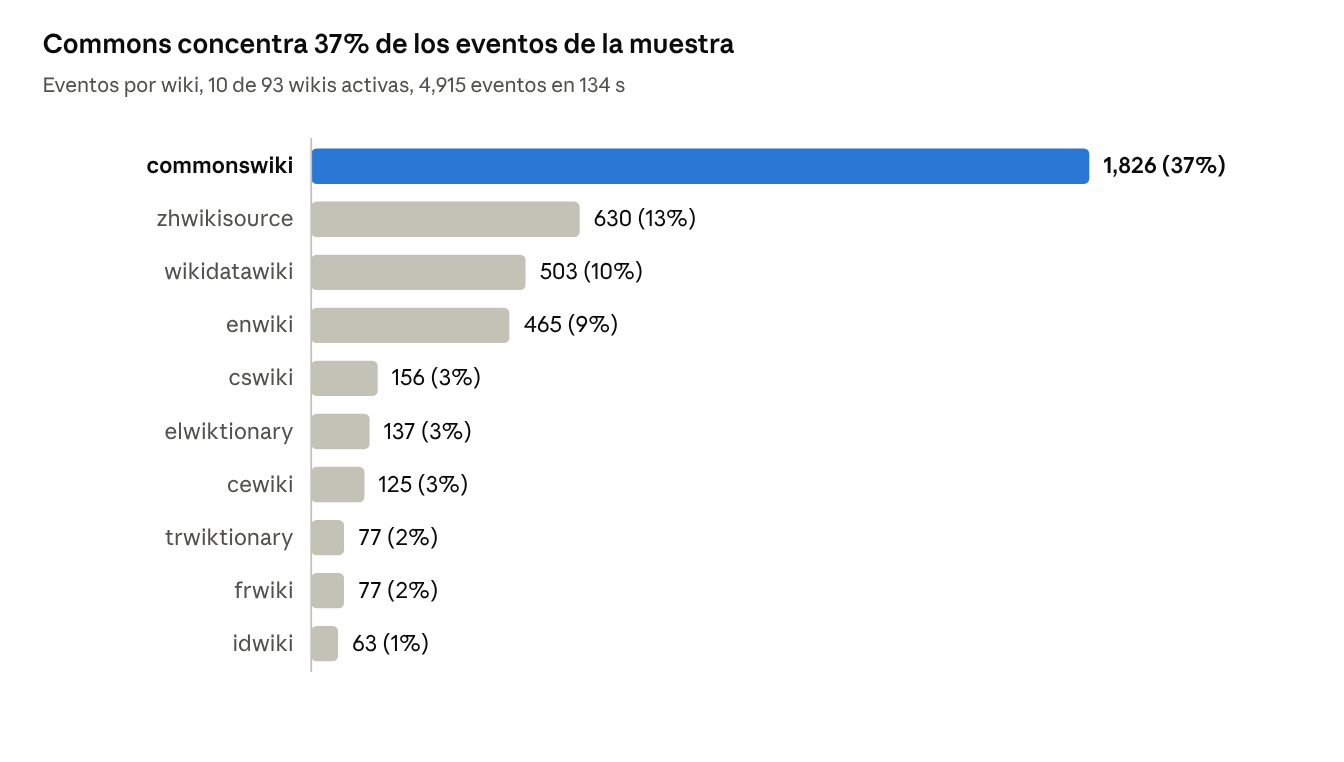
\includegraphics[width=0.93\textwidth]{eventos-por-wiki.png}
\caption{Distribución por wiki en la captura exploratoria multilingüe.}
\fuente{imagen y muestra del 31 de octubre incluidas en \ruta{docs/justificacion-dataset.md}}
\end{figure}

Para el alcance final, la bitácora registra ventanas de 16\,442 y 15\,402 eventos en dos horas del 31 de octubre. Más adelante se documentaron millones de eventos acumulados; sin embargo, ese historial fue recortado durante la migración del 17 de noviembre. Después de la reconstrucción se reportaron 206\,762 eventos desde las 01:00 UTC de ese día, equivalentes a 4.14 veces el mínimo requerido \cite{bitacora}. Es una cifra documentada de ese corte y no una consulta en vivo realizada durante la redacción.

\section{Validación, deduplicación y enriquecimiento}
La función \codigo{validate} devuelve un motivo explícito cuando un documento incumple las reglas. Se comprueba la presencia de campos, los tipos de texto, el \codigo{namespace} entero, el booleano \codigo{bot}, la fecha, la estructura de \codigo{length} y ciertos parámetros de registro. La validación de \codigo{timestamp} exige su presencia; la asignación temporal del procesamiento utiliza \codigo{meta.dt}.

La limpieza escribe dos archivos comprimidos: eventos aceptados y rechazados con su motivo. Un conjunto de identificadores evita duplicados dentro del archivo. Los documentos aceptados reciben \codigo{_id=meta.id} y un bloque \codigo{derived}. Los campos originales se mantienen salvo la normalización de claves que aplica la carga documental.

\begin{tabla}
\begin{tabularx}{\textwidth}{P{4.0cm}Y}
\toprule
Campo derivado & Uso \\
\midrule
\codigo{event_time}, \codigo{event_dt} & Momento normalizado en UTC; texto ISO y fecha BSON respectivamente. \\
\codigo{date}, \codigo{hour}, \codigo{minute} & Construcción de ventanas y series temporales. \\
\codigo{user_type} & Clasificación en bot, temporal, IP o registrado. \\
\codigo{page_key} & Identidad \codigo{wiki:title} para evitar mezclar páginas de wikis distintas. \\
\codigo{delta_bytes} & Diferencia entre tamaño nuevo y anterior en \codigo{edit} y \codigo{new}. \\
\codigo{revert_target}, \codigo{message_target} & Destinatarios inferidos de reversiones y mensajes. \\
Campos de categorías y registros & Página categorizada, acción, bloqueo, agradecimiento, traslado o archivo. \\
\bottomrule
\end{tabularx}
\caption{Enriquecimiento de los documentos aceptados.}
\end{tabla}

\subsection{Clasificación de editores}
Se considera bot a un evento marcado como tal, a una cuenta cuyo nombre satisface la expresión regular de bot o a una cuenta incluida en \codigo{KNOWN_BOTS}, como Automoderador. Las cuentas que comienzan con \texttt{\textasciitilde} se clasifican como temporales; los nombres que representan una IP se identifican con \codigo{ipaddress}; los restantes se consideran registrados. Es una regla práctica cuya precisión no fue medida con un conjunto de etiquetas independiente.

\subsection{Detección de reversiones y relaciones}
Una reversión requiere un enlace a contribuciones de otro editor y palabras de reversión en inglés o español. Se excluyen avisos con \codigo{Warning}, \codigo{Reporting}, restauraciones con \codigo{Restored} y autorreversiones. Los mensajes se infieren de ediciones en el espacio de discusión de usuarios, \codigo{namespace=3}. La categorización combina el enlace a la página con frases de adición o eliminación.

Estas reglas ofrecen evidencia de actividad de revisión, pero pueden omitir formatos de comentario no contemplados. Un \codigo{revert_target} es un resultado heurístico, no una etiqueta definitiva de vandalismo.

\section{Calidad y límites de cobertura}
La calidad se calcula como eventos válidos únicos divididos entre entradas leídas por la limpieza. Los duplicados se contabilizan aparte, pero permanecen en el denominador; por ello pueden reducir el porcentaje sin ser rechazos. Los registros descartados antes de formar el archivo, como otras wikis o eventos sin fecha interpretable durante la extracción, quedan fuera de ese indicador.

Un resultado de 100\,\% significa que todas las entradas consideradas pasaron las reglas y la deduplicación. No demuestra cobertura total del stream, ausencia de sesgo, exactitud semántica ni disponibilidad continua. La cobertura se administra por separado con tramos persistidos y recuperación de ventanas.

\chapter{ARQUITECTURA Y MODELOS DE DATOS}
\label{cap:modelos}
\section{Arquitectura general}
La solución combina una capa rápida con una capa por lotes y materializaciones orientadas a consulta. La capa rápida conserva cambios recientes y permite seguimiento provisional. La capa por lotes procesa horas completas y construye los resúmenes y relaciones que requieren consolidación. Ambas comparten MongoDB como repositorio de eventos \cite{repo}.

La figura~\ref{fig:arquitectura} resume el flujo implementado. No se utiliza Spark ni un clúster Kafka propio: el equipo consume el endpoint SSE publicado por Wikimedia. PostgreSQL almacena metadatos de Airflow y no sustituye a ninguna de las tres bases analíticas.

\begin{figure}[htbp]
\centering
\begin{tikzpicture}[node distance=0.9cm and 0.6cm]
\node[caja,fill=azul,text width=5.1cm] (src) {Wikimedia EventStreams\\\footnotesize recentchange: enwiki y eswiki};
\node[caja,below left=0.9cm and -1.1cm of src,text width=3.5cm] (stream) {Streaming continuo\\\footnotesize buffer: 2 s o 200 eventos};
\node[caja,below right=0.9cm and -1.1cm of src,text width=3.5cm] (air) {Airflow cada hora\\\footnotesize extracción y consolidación};
\node[caja,below=1.2cm of stream,fill=azul,text width=3.5cm] (mongo) {MongoDB\\\footnotesize eventos y coordinación};
\node[caja,below=1.2cm of air,fill=rosa,text width=3.5cm] (neo) {Neo4j\\\footnotesize contribuciones temporales};
\node[caja,below=1.15cm of $(mongo)!0.5!(neo)$,text width=4.2cm] (cass) {Cassandra\\\footnotesize minutos, horas, rankings y KPIs};
\node[caja,below=0.9cm of cass,text width=4.2cm,fill=azul] (api) {FastAPI $\rightarrow$ React / nginx\\\footnotesize consultas, CRUD y visualización};
\draw[flecha] (src) -- (stream);
\draw[flecha,dashed] (src) -- node[right,font=\scriptsize]{respaldo} (air);
\draw[flecha] (stream) -- (mongo);
\draw[flecha] (mongo) -- node[above,font=\scriptsize,sloped]{hora completa} (air);
\draw[flecha] (air) -- (neo);
\draw[flecha] (air.west) -- ++(-0.45,0) |- (cass.east);
\draw[flecha] (stream.west) -- ++(-0.55,0) |- node[near end,below,font=\scriptsize]{minutos provisionales} (cass.west);
\draw[flecha] (cass) -- (api);
\draw[flecha] (mongo.west) -- ++(-0.85,0) |- (api.west);
\draw[flecha] (neo.east) -- ++(0.85,0) |- (api.east);
\end{tikzpicture}
\caption{Flujo lógico de la arquitectura implementada.}\label{fig:arquitectura}
\fuente{elaboración propia a partir del código del repositorio; línea discontinua: recuperación externa}
\end{figure}

\section{Justificación de la persistencia multimodelo}
La distribución se decide según el patrón de acceso. MongoDB conserva documentos heterogéneos y permite inspeccionar campos anidados. Cassandra guarda respuestas temporales precalculadas. Neo4j representa relaciones y soporta recorridos entre editores y páginas. El resultado es una persistencia políglota: los modelos complementan sus funciones y requieren sincronización explícita.

\begin{tabla}
\begin{tabularx}{\textwidth}{P{2.3cm}YY}
\toprule
Base & Información principal & Consulta que motiva el modelo \\
\midrule
MongoDB & Evento completo normalizado, derivados, rechazos y control. & Buscar una edición y explicar su contexto o reconstruir una ventana. \\
Cassandra & Series, resúmenes, actividad por editor, rankings y KPIs. & Recuperar una serie por wiki y día o los valores horarios de un indicador. \\
Neo4j & Entidades e interacciones con atribución temporal. & Hallar coeditores, patrulleros y reversiones recibidas. \\
\bottomrule
\end{tabularx}
\caption{Distribución de responsabilidades entre las tres bases.}
\end{tabla}

La ventaja no elimina los costos: existen datos derivados duplicados, tres conexiones y reglas de reconstrucción. La consistencia entre bases se consigue mediante ejecuciones y reintentos; no existe una transacción distribuida que confirme MongoDB, Cassandra y Neo4j al mismo tiempo.

\section{MongoDB: documentos y fuente de reconstrucción}
\subsection{Colecciones}
El esquema se define en \ruta{db/mongo/schema.json} y se aplica con \codigo{ensure_schema}. La colección \codigo{events} almacena un documento por \codigo{meta.id}. Los \textit{upserts} usan \codigo{ReplaceOne} y lotes de 1\,000 operaciones. Los campos originales no se proyectan fuera de este almacenamiento; sin embargo, \codigo{sanitize} cambia puntos por guiones bajos y retira prefijos de dólar en las claves. En una extracción directa de EventStreams, el archivo crudo conserva la representación de origen. Si la hora se exporta desde MongoDB, sus claves ya están normalizadas.

\begin{tabla}
\begin{tabularx}{\textwidth}{P{4.0cm}Y}
\toprule
Colección & Función \\
\midrule
\codigo{events} & Documentos aceptados, campos originales normalizados y \codigo{derived}. \\
\codigo{events_rejected} & Evento o entrada rechazada, motivo e instante cuando es interpretable. \\
\codigo{pipeline_runs} & Resultado por ventana, cargas, KPIs, versión y fecha de publicación. \\
\codigo{stream_state} & Marcador SSE para retomar el consumo. \\
\codigo{stream_cobertura} & Tramos de actividad continua que habilitan la lectura horaria local. \\
\codigo{pipeline_windows} & Bloqueo renovable, marca de escritura y manifiestos de reconstrucción. \\
\bottomrule
\end{tabularx}
\caption{Colecciones del esquema documental.}
\end{tabla}

\subsection{Validador e índices}
MongoDB permite combinar esquema flexible con validaciones de tipos y campos \cite{mongo}. En el proyecto, el validador exige identificador, tipo, wiki, título, usuario, metadatos y derivados. Dentro de \codigo{derived}, la fecha BSON, el día, la hora, el tipo de usuario y la clave de página son obligatorios. Se configura \codigo{validationLevel=moderate}; la validación Python realiza comprobaciones adicionales antes de la carga.

Hay índices por fecha; por wiki, tipo y fecha; por editor y fecha; por página; por editor revertido; y por wiki, fecha e identificador. Este último permite ordenar de forma estable cuando varios eventos tienen el mismo instante. Los rechazos se indexan por motivo y fecha; las ejecuciones por inicio de ventana.

\par\noindent\begin{minipage}{\linewidth}
\begin{lstlisting}[caption={Consulta documental por wiki y ventana; ejemplo de uso.}]
db.events.find({
  wiki: "eswiki",
  "derived.event_dt": {
    $gte: ISODate("2026-11-17T10:00:00Z"),
    $lt:  ISODate("2026-11-17T11:00:00Z")
  }
}).sort({"derived.event_dt": -1, _id: -1})
\end{lstlisting}
\end{minipage}\par

\section{Cassandra: modelo orientado a consultas}
El diseño sigue el acceso esperado: una partición y un rango temporal permiten leer los resultados de una vista. La documentación de Cassandra describe este modelado como orientado a consultas, con desnormalización en función de los patrones de lectura \cite{cassandra}. El proyecto materializa ocho tablas en \ruta{db/cassandra/schema.cql}.

\begin{tabla}
\begin{tabularx}{\textwidth}{P{4.0cm}P{3.1cm}Y}
\toprule
Tabla & Partición; orden interno & Uso \\
\midrule
\codigo{resumen_por_hora} & \codigo{fecha}; \codigo{hora,wiki} & Conteos horarios por wiki y tipo, editores, reversiones y bytes. \\
\codigo{eventos_por_minuto} & \codigo{wiki,fecha}; \codigo{minuto} descendente & Serie temporal provisional y consolidada. \\
\codigo{actividad_editor} & \codigo{editor}; \codigo{fecha,hora,wiki} & Historial de una cuenta. \\
\codigo{paginas_top_por_hora} & \codigo{wiki,fecha}; \codigo{hora,posicion} & Hasta 20 páginas por hora, ordenadas por editores y ediciones. \\
\codigo{paginas_disputadas_por_hora} & \codigo{wiki,fecha}; \codigo{hora,posicion} & Hasta 20 páginas con más reversiones por hora. \\
\codigo{kpis} & \codigo{kpi}; \codigo{ventana} descendente & Serie global de cada indicador. \\
\codigo{kpis_por_wiki} & \codigo{kpi,wiki}; \codigo{ventana} descendente & Serie filtrada por comunidad. \\
\codigo{ejecuciones} & \codigo{fecha}; \codigo{ventana} descendente & Calidad, volumen, duración y fuente de extracción. \\
\bottomrule
\end{tabularx}
\caption{Tablas, particiones y accesos en Cassandra.}\label{tab:cassandra}
\end{tabla}

Las columnas almacenan valores calculados, no incrementos de contadores CQL. Reprocesar reemplaza la ventana y escribe el resultado absoluto, lo que evita volver a sumar el mismo evento. El ranking de páginas activas prioriza editores distintos, luego ediciones y título; el ranking de disputa prioriza reversiones.

\par\noindent\begin{minipage}{\linewidth}
\begin{lstlisting}[caption={Lectura de una serie temporal por su partición.}]
SELECT minuto, eventos, eventos_bot, reversiones
FROM wikipipe.eventos_por_minuto
WHERE wiki = 'eswiki' AND fecha = '2026-11-17'
  AND minuto >= '2026-11-17T10:00:00Z'
  AND minuto <  '2026-11-17T11:00:00Z';
\end{lstlisting}
\end{minipage}\par

El keyspace usa \codigo{SimpleStrategy} con factor de replicación 1. Esta elección es compatible con una demostración de un nodo, pero no ofrece tolerancia a la pérdida de ese nodo. Además, las particiones por editor y por KPI crecen con el historial; una operación prolongada requeriría segmentarlas, por ejemplo, por mes.

\section{Neo4j: relaciones y atribución temporal}
\subsection{Entidades e identidad}
El modelo analítico contiene cuatro clases de nodo. \codigo{Editor} usa \codigo{user} como identidad global; \codigo{Pagina} y \codigo{Categoria} usan una clave con wiki y nombre; \codigo{Wiki} usa su nombre. Un nodo auxiliar \codigo{PipelineModelo} almacena la versión y actúa como punto de bloqueo de las cargas transaccionales.

La unicidad de \codigo{Editor.user} implica que una cuenta con el mismo nombre en las dos wikis se trata como la misma identidad. Este supuesto es relevante al contar personas distintas: el sistema observa cuentas y nombres, no verifica identidades reales.

\begin{figure}[htbp]
\centering
\begin{tikzpicture}
\node[caja,fill=azul,text width=2.8cm] (a) at (0,3.3) {Editor A\\\footnotesize user único};
\node[caja,fill=rosa,text width=2.8cm] (b) at (7.6,3.3) {Editor B\\\footnotesize user único};
\node[caja,text width=2.8cm] (p) at (0,0.5) {Página\\\footnotesize key = wiki:título};
\node[caja,text width=2.8cm] (c) at (7.6,0.5) {Categoría\\\footnotesize\texttt{wiki:nombre}};
\node[caja,text width=2.8cm] (w) at (3.8,-2.4) {Wiki\\\footnotesize nombre único};
\draw[flecha] (a) -- node[above,font=\scriptsize,align=center,text width=4cm]{REVIRTIO / MENSAJE\_A\\AGRADECIO / BLOQUEO} (b);
\draw[flecha] (a) -- node[left,font=\scriptsize,align=right]{EDITO / CREO\\SUBIO} (p);
\draw[flecha] (b) -- node[above,font=\scriptsize,sloped]{EDITO} (p);
\draw[flecha] (p) -- node[above,font=\scriptsize]{EN\_CATEGORIA} (c);
\draw[flecha] (p) -- node[pos=.55,left,font=\scriptsize]{PERTENECE\_A} (w);
\draw[flecha] (c) -- node[pos=.55,right,font=\scriptsize]{PERTENECE\_A} (w);
\end{tikzpicture}
\caption{Núcleo del grafo analítico y relaciones principales.}\label{fig:grafo}
\fuente{elaboración propia; las contribuciones de actividad conservan wiki y ventana}
\end{figure}

\subsection{Relaciones de actividad y estado}
\begin{tabla}
\begin{tabularx}{\textwidth}{P{3.3cm}P{3.0cm}Y}
\toprule
Relación & Origen y destino & Significado \\
\midrule
\codigo{EDITO}, \codigo{CREO}, \codigo{SUBIO} & Editor $\to$ Página & Ediciones y creaciones; subida de archivo. \codigo{EDITO} incluye también eventos \codigo{new}. \\
\codigo{REVIRTIO}, \codigo{MENSAJE_A} & Editor $\to$ Editor & Reversiones y mensajes inferidos. \\
\codigo{AGRADECIO}, \codigo{BLOQUEO} & Editor $\to$ Editor & Acción de registro con destinatario. \\
\codigo{MOVIDA_A} & Página $\to$ Página & Traslado con título de destino. \\
\codigo{PERTENECE_A} & Página/Categoría $\to$ Wiki & Comunidad de pertenencia. \\
\codigo{CAMBIO_CATEGORIA} & Página $\to$ Categoría & Contribución temporal de adición o eliminación. \\
\codigo{EN_CATEGORIA} & Página $\to$ Categoría & Estado derivado de la última acción conservada. \\
\codigo{ACTIVO_EN} & Editor $\to$ Wiki & Actividad temporal para reconstruir atributos de la cuenta. \\
\codigo{COEDITA} & Editor $\leftrightarrow$ Editor & Relación materializada entre humanos con páginas comunes. \\
\bottomrule
\end{tabularx}
\caption{Relaciones del modelo temporal implementado.}
\end{tabla}

Las relaciones de contribución incluyen \codigo{ventana}, \codigo{wiki} y \codigo{version=2}. Por ello, dos editores pueden tener varias relaciones del mismo tipo en horas o wikis diferentes. Una consulta debe sumar \codigo{veces} y aplicar el período correspondiente; contar aristas sin considerar su granularidad produciría una métrica distinta.

Las cargas usan \codigo{UNWIND} y \codigo{MERGE}. Este último permite buscar o crear patrones; la unicidad se refuerza con restricciones explícitas \cite{neo4j}. Cada hora se reemplaza en una sola transacción, y después se recalculan atributos y relaciones acumuladas afectadas.

\subsection{Coedición y límites del modelo}
La relación materializada \codigo{COEDITA} se genera para páginas con entre 2 y 50 editores humanos, para limitar la explosión de pares. Es una relación acumulada sin wiki. En cambio, el KPI horario de editor más conectado recorre directamente \codigo{EDITO} con filtros de hora, wiki y tipo humano; no depende de ese límite de materialización. La API también calcula coeditores desde \codigo{EDITO} cuando necesita un filtro por wiki.

Compartir páginas expresa proximidad de actividad, no necesariamente cooperación. Además, categorías, bloqueos y traslados reflejan los eventos conservados; el sistema no reconstruye un estado completo de Wikipedia anterior al inicio de la captura. Las relaciones \codigo{CREO}, \codigo{SUBIO} y \codigo{MOVIDA_A} amplían el modelo, aunque todavía no alimentan un KPI específico del dashboard.

\chapter{AUTOMATIZACIÓN, CONSISTENCIA Y DESPLIEGUE}
\label{cap:pipeline}
\section{Capa rápida: ingesta continua}
El servicio \codigo{stream} ejecuta \codigo{python -m wikipipe.streaming}. Cada evento recibido se filtra por wiki, se valida y se enriquece. El consumidor acumula eventos hasta 200 registros o hasta que transcurran aproximadamente dos segundos desde el último vaciado. Estos parámetros determinan una frecuencia objetivo; la duración real también depende de las escrituras, bloqueos y conexiones.

Los documentos se guardan primero en MongoDB mediante \textit{upsert}. Los minutos afectados se reconstruyen leyendo los eventos persistidos y se escriben como valores absolutos en Cassandra. Así, reiniciar el proceso o recibir nuevamente un evento no exige confiar en un contador en memoria. Los minutos pendientes se conservan como pendientes cuando una escritura falla.

El marcador SSE se persiste en \codigo{stream_state}. Al reiniciar se usa \codigo{Last-Event-ID}, salvo que el marcador tenga más de 24 horas, en cuyo caso el consumidor comienza en vivo. El código incorpora reconexión con espera creciente. Una parada prolongada requiere verificar y recuperar las ventanas faltantes.

\section{Selección de la fuente horaria}
El módulo \codigo{fuente.py} decide entre MongoDB y EventStreams. MongoDB se usa cuando un tramo de cobertura comienza antes o en el inicio de la ventana y se extiende hasta cinco minutos después de su cierre. El margen ayuda a evitar lecturas prematuras; solo se exportan eventos dentro del intervalo solicitado.

Si el tramo sigue activo pero todavía no alcanza el margen, se sondea cada 15 segundos hasta un máximo de diez minutos. Un tramo cuya actualización supera dos minutos se considera detenido. Si falta cobertura, se solicita nuevamente la hora al stream externo.

La cobertura avanza únicamente después de persistir eventos y con fechas recibidas con menos de 60 segundos de retraso. Este control reduce el riesgo de declarar completa una hora mientras el consumidor recupera atrasos. No es una garantía matemática de ausencia de eventos tardíos arbitrarios.

\section{DAG de Apache Airflow}
El DAG \codigo{wikipedia_recent_changes} utiliza \codigo{@hourly}, \codigo{catchup=False} y \codigo{max_active_runs=1}. Cada tarea dispone de dos reintentos con cinco minutos de espera; la extracción tiene un límite de ejecución de 30 minutos. La ventana se toma de \codigo{data_interval_start} y \codigo{data_interval_end}, según el modelo de intervalos de Airflow \cite{airflow}.

\begin{figure}[htbp]
\centering
\begin{tikzpicture}[node distance=0.65cm and 0.65cm]
\node[caja,text width=5.0cm,fill=azul] (e) {1. extraer};
\node[caja,below=of e,text width=5.0cm] (v) {2. validar\_y\_limpiar};
\node[caja,below=of v,text width=5.0cm] (m) {3. cargar\_mongo};
\node[caja,below left=0.8cm and -1.1cm of m,text width=3.7cm] (c) {4. cargar\_cassandra};
\node[caja,below right=0.8cm and -1.1cm of m,text width=3.7cm] (n) {5. cargar\_neo4j};
\node[caja,below=1.0cm of $(c)!0.5!(n)$,text width=5.0cm,fill=rosa] (k) {6. calcular\_kpis};
\draw[flecha] (e)--(v);\draw[flecha] (v)--(m);
\draw[flecha] (m)--(c);\draw[flecha] (m)--(n);
\draw[flecha] (c)--(k);\draw[flecha] (n)--(k);
\end{tikzpicture}
\caption{Dependencias de las seis tareas del DAG horario.}\label{fig:dag}
\fuente{\ruta{airflow/dags/wikipedia_pipeline.py}}
\end{figure}

\subsection{Entradas, transformaciones y salidas}
\begin{enumerate}
\item \textbf{Extraer.} Exporta la ventana desde MongoDB o la solicita a EventStreams. Escribe \ruta{data/raw/AAAA-MM-DD/HHMM.jsonl.gz}, inicialmente con un nombre temporal que se reemplaza al terminar.
\item \textbf{Validar y limpiar.} Comprueba reglas, elimina duplicados del archivo, calcula \codigo{derived} y genera archivos válidos y rechazados con estadísticas globales y por wiki.
\item \textbf{Cargar MongoDB.} Inserta o reemplaza los eventos limpios y los rechazos. Si la fuente fue MongoDB, omite la reescritura porque los eventos ya están almacenados.
\item \textbf{Cargar Cassandra.} Lee de MongoDB la ventana y construye conteos, series, actividad por cuenta y rankings. Reemplaza las filas anteriores bajo un bloqueo horario.
\item \textbf{Cargar Neo4j.} Lee la misma ventana, construye filas de entidades y relaciones y reemplaza sus contribuciones en una transacción. Puede ejecutarse en paralelo con Cassandra.
\item \textbf{Calcular KPIs.} Espera las dos cargas. Calcula los indicadores globales y por wiki, los escribe en Cassandra, registra la ejecución y publica un resumen de versión 2 en MongoDB. También actualiza acumulados posteriores y el crecimiento de la siguiente hora cuando corresponde.
\end{enumerate}

\section{Tiempo, reintentos e idempotencia}
Se usan intervalos semiabiertos:
\[
W_h=\{e\mid h\leq t_e<h+1\text{ hora}\}.
\]
Así, un evento situado exactamente en el cierre pertenece a la hora siguiente. Las ventanas se identifican en UTC. La API convierte las fechas de consulta diaria a UTC$-5$ para su presentación y puede necesitar leer dos días UTC para formar un día local.

La extracción externa no dispone de parámetro de cierre. El código observa el avance de los dos centros de datos configurados, \codigo{codfw} y \codigo{eqiad}, con un margen de 120 segundos, un umbral de eventos posteriores y un criterio de inactividad. Es una política operativa para cerrar el consumo; una demora excepcional más larga puede requerir reconciliación posterior.

\subsection{Coordinación de escrituras en Cassandra}
Streaming y Airflow comparten \codigo{lock_hour}, implementado con un documento en MongoDB. El bloqueo vence a los 60 segundos, se renueva cada 15 y genera una marca creciente en microsegundos. Las eliminaciones usan esa marca y las inserciones la marca más uno. De esta manera, una escritura atrasada de un propietario vencido no debe sobrescribir un resultado más reciente.

Antes de escribir, Cassandra conserva un manifiesto de editores anteriores y pendientes. Al reintentar puede borrar tanto filas históricas de esa hora como filas de una carga parcial. La reconstrucción reemplaza también los minutos y los rankings, y crea resúmenes de cero para wikis sin eventos en la ventana.

\subsection{Reemplazo del grafo y publicación}
Neo4j elimina las contribuciones de versión 2 de la hora y escribe las nuevas dentro de una transacción. El nodo \codigo{PipelineModelo} serializa estas reconstrucciones. Si falla la transacción, se conserva el estado previo; si termina, se actualizan estados afectados, categorías y coedición.

El registro de una ejecución completada es la señal para publicar sus KPIs. La API consulta ventanas de versión 2 que no estén marcadas como \codigo{reprocessing}. Además, compara \codigo{recorded_at} antes y después de lecturas de resultados y descarta ventanas que cambiaron durante la consulta. Es una estrategia de publicación y consistencia eventual, no una transacción conjunta entre motores.

Una corrección o eliminación en MongoDB necesita reprocesar la ventana para reflejarse en las bases derivadas. La tarea \codigo{cargar_mongo} omite la reescritura cuando exportó desde MongoDB; por ello, un cambio futuro en las reglas de enriquecimiento exige una migración explícita de \codigo{derived}, no solo volver a ejecutar esa ruta.

\section{Contenedores e infraestructura}
Docker Compose define MongoDB 7.0.14, Cassandra 4.1.7, Neo4j Community 5.26.2, PostgreSQL 16.4, Airflow 2.10.5, streaming, API y web. Se usan volúmenes para las bases y una carpeta persistente para los archivos del pipeline. Los \textit{health checks}, políticas de reinicio y límites de memoria ayudan a ordenar el arranque y contener fallos.

Terraform crea una VM de Compute Engine, IP estática, bucket de Cloud Storage, cuenta de servicio y reglas de firewall. La configuración predeterminada utiliza una VM \codigo{e2-standard-2}, con 2 vCPU y 8 GB de RAM, y un disco inicial de 50 GB. La bitácora documenta su ampliación posterior a 100 GB; el archivo Terraform conserva el valor inicial y excluye ese cambio del ciclo de recreación \cite{bitacora}.

El arranque instala Docker, obtiene el código y las variables y ejecuta Compose. Los archivos crudos se sincronizan al bucket cada 30 minutos. Ese respaldo no representa, por sí solo, una copia consistente de los volúmenes de las tres bases.

\subsection{Acceso y despliegue continuo}
Las interfaces administrativas se restringen por CIDR, SSH utiliza IAP y el dashboard dispone de contraseña compartida. En GCP no se crean reglas públicas para MongoDB y Cassandra. En local, Compose publica sus puertos, por lo que el entorno tiene un perímetro distinto.

El timer de \codigo{autodeploy.sh} compara \codigo{main} cada minuto, construye las imágenes en una carpeta temporal y sincroniza el código si la compilación termina. Conserva \codigo{.env} y \codigo{data/} y reinicia API y streaming. Compilar antes de actualizar reduce fallos de construcción, pero no valida compatibilidad de esquemas ni ejecuta automáticamente una migración de datos. El incidente del modelo 2 mostró la necesidad de agregar esa validación al despliegue.

\chapter{API, OPERACIONES CRUD Y DASHBOARD}
\label{cap:aplicacion}
\section{Capa de consulta y acceso}
El dashboard usa React, TypeScript, componentes shadcn/ui, Recharts y un grafo interactivo. nginx sirve la aplicación y redirige \codigo{/api} a FastAPI. El navegador no abre conexiones directas con las bases: la API centraliza consultas, conversiones temporales y operaciones de escritura \cite{repo}.

El módulo \ruta{api/queries.py} conserva conexiones y utiliza una caché breve para consultas repetidas. Las mutaciones CRUD limpian esa caché. Los filtros se validan en el servidor; los valores entran como parámetros a las consultas y los tipos de relación y columnas editables se restringen mediante listas permitidas.

Cuando \codigo{DASHBOARD_PASSWORD} está definida, la API requiere una cookie de sesión para las rutas protegidas. La clave es compartida por el equipo; el código no implementa cuentas individuales ni permisos por rol. La cookie usa \codigo{HttpOnly} y \codigo{SameSite=Lax}. Los archivos de despliegue revisados no incluyen terminación TLS, por lo que un uso fuera de la demostración requiere completar esa protección y la administración de identidades.

\section{Operaciones CRUD en MongoDB}
La interfaz ofrece formulario y JSON sincronizados para crear eventos de los cuatro tipos. El servidor calcula \codigo{derived}; el usuario no necesita escribirlo manualmente. Un documento incompleto permite demostrar el rechazo del validador. Los duplicados de \codigo{_id} se informan como conflicto.

La consulta admite wiki, tipo, editor, título, período, demostración e identificador. El detalle expone el documento. En una actualización se aceptan rutas como \codigo{length.new}; se protegen \codigo{_id}, \codigo{meta.id} y \codigo{derived}. El servidor simula el nuevo documento, recalcula los derivados necesarios y retira los campos derivados que ya no correspondan.

La eliminación muestra el registro y requiere confirmación en la interfaz. Modificar un evento cambia MongoDB de inmediato, pero no reconstruye automáticamente Cassandra y Neo4j; el usuario operador debe reprocesar las horas afectadas para actualizar resultados consolidados.

\begin{figure}[H]
\centering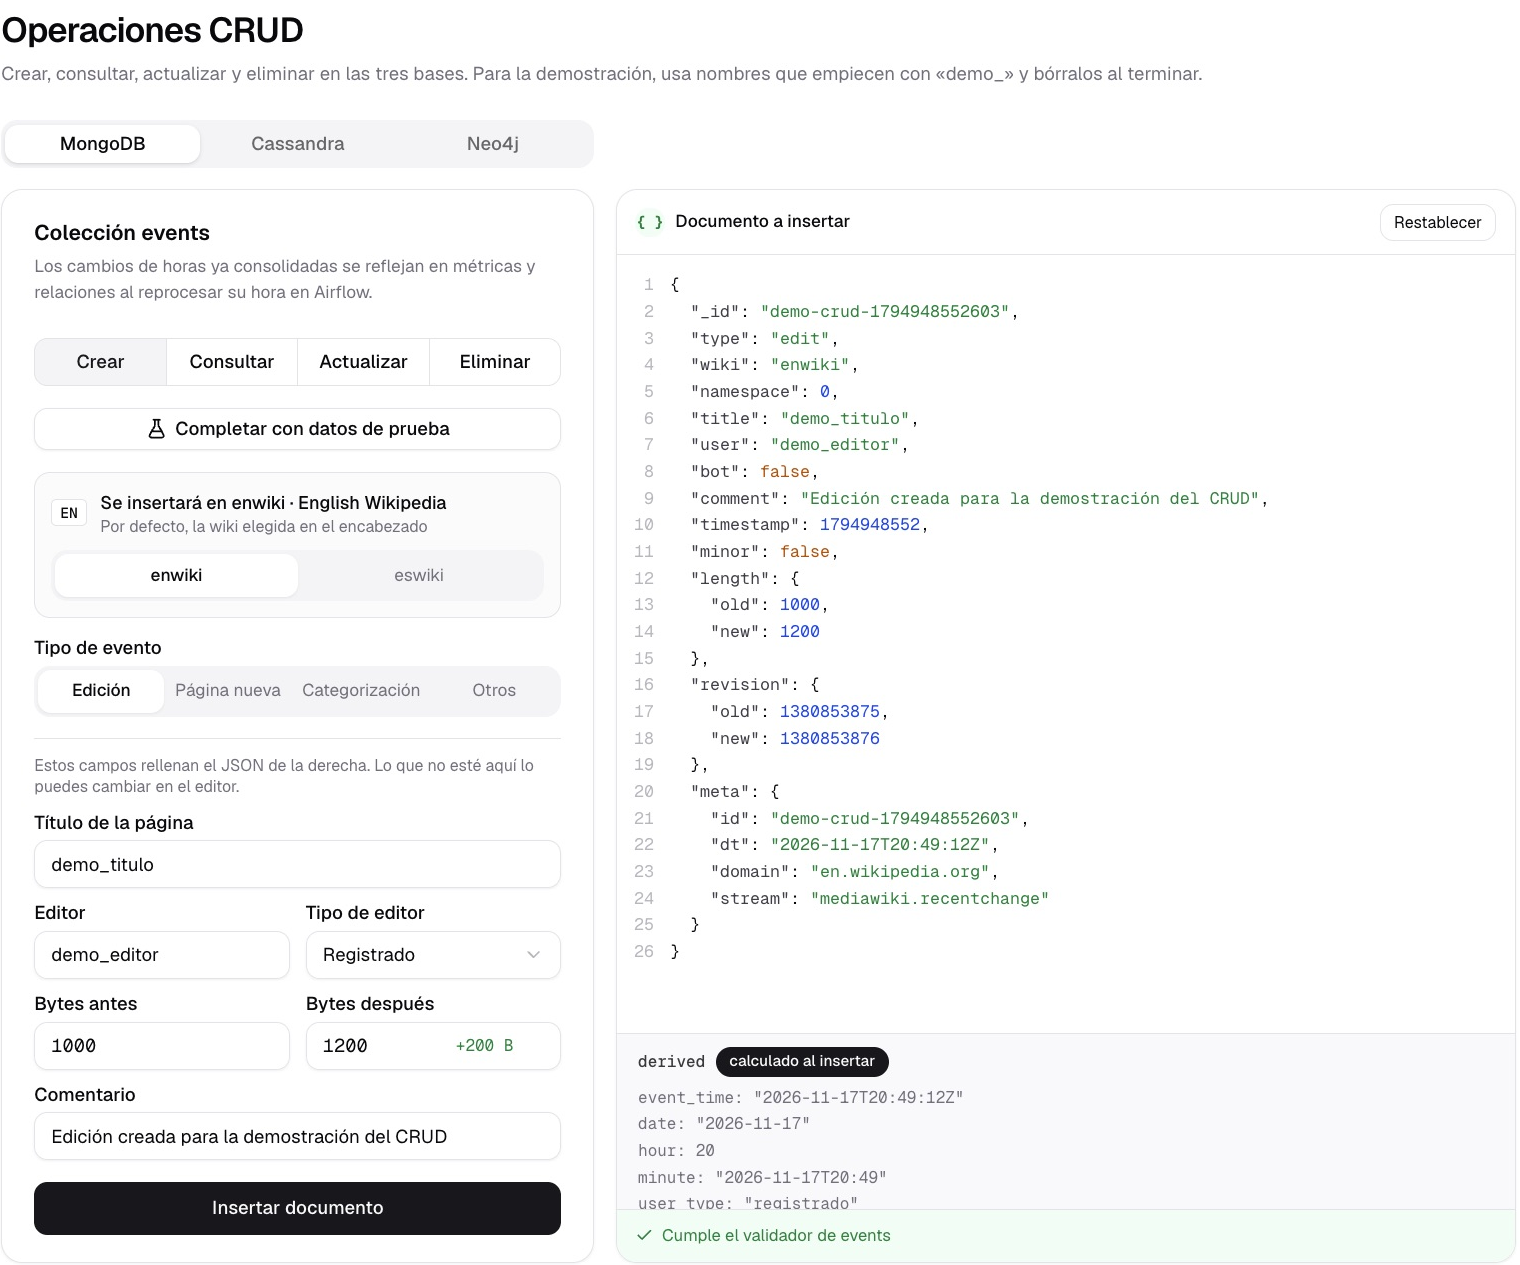
\includegraphics[width=0.94\textwidth,height=0.62\textheight,keepaspectratio]{dashboard-crud-mongo.png}
\caption{MongoDB: formulario y documento JSON de una creación.}\label{fig:ui-mongo}
\fuente{dashboard del proyecto desplegado en Google Cloud Platform}
\end{figure}

\section{Operaciones CRUD en Cassandra}
El CRUD vigente trabaja sobre \codigo{kpis}, cuya clave completa es \codigo{(kpi,ventana)}. La inserción permite crear una fila y también reemplazar una clave existente. La consulta accede a una partición y opcionalmente a un día y una hora UTC. La API normaliza la ventana al inicio horario.

La actualización admite únicamente \codigo{valor} y \codigo{detalle}, verifica que la fila exista y rechaza valores incompatibles. Esta comprobación evita que un \codigo{UPDATE} sobre una clave ausente se interprete en la interfaz como modificación de un registro previo. Se puede eliminar una fila con la clave completa o toda la partición si solo se indica el KPI.

Se recomienda utilizar nombres \codigo{demo_} en la exposición. El código actual reconoce ese prefijo para organizar registros de demostración, pero no impone una prohibición general de escribir otros nombres. Algunas notas históricas describen una restricción anterior que ya no corresponde al comportamiento actual.

\begin{figure}[H]
\centering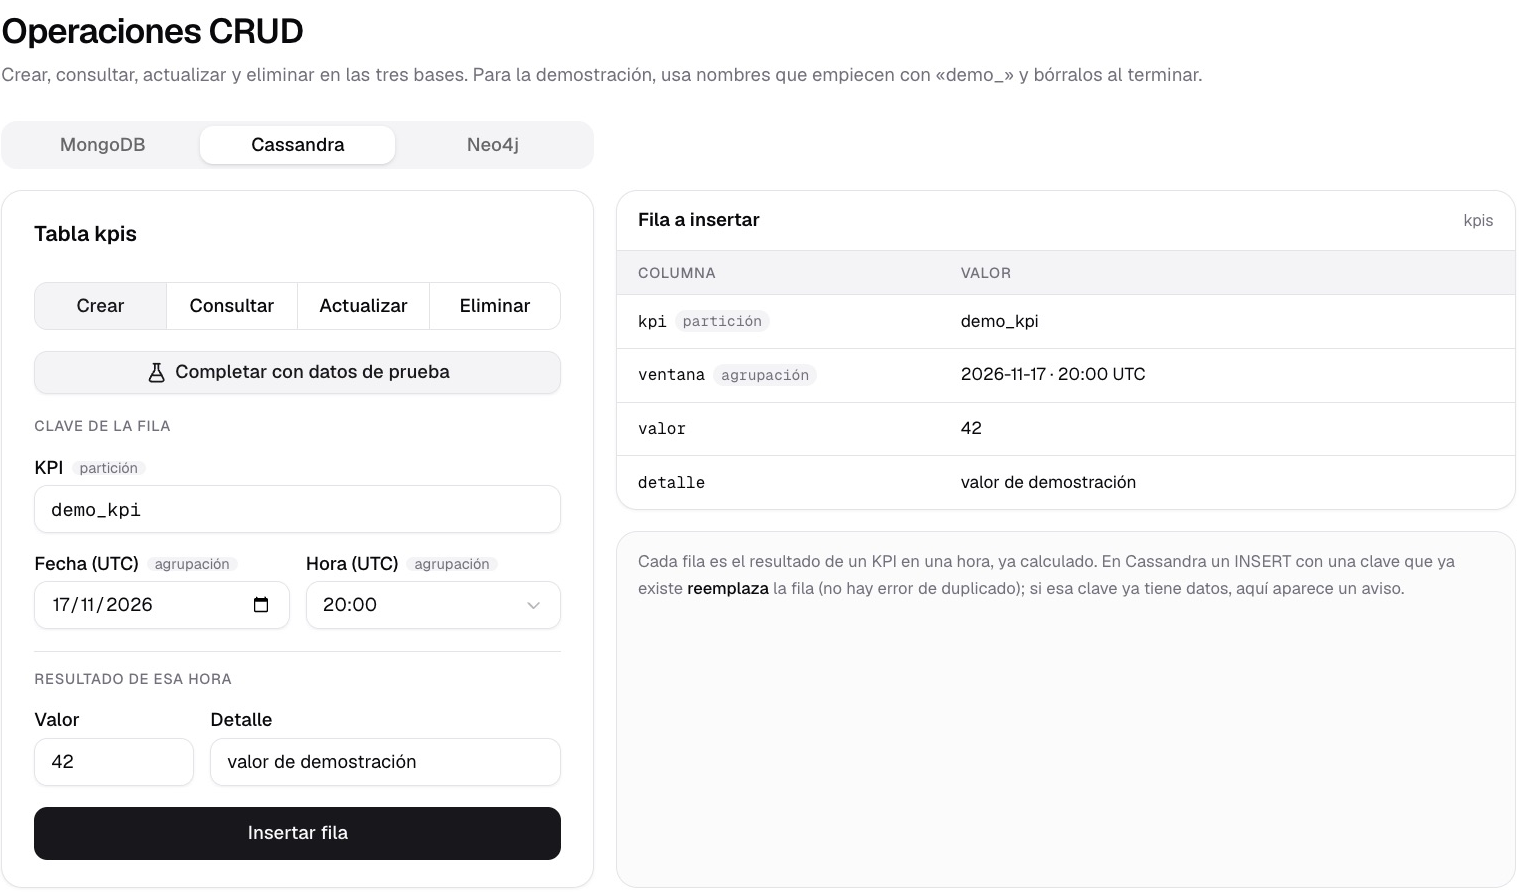
\includegraphics[width=0.96\textwidth,height=0.57\textheight,keepaspectratio]{dashboard-crud-cassandra.png}
\caption{Cassandra: clave, valor y vista previa de una fila de KPI.}\label{fig:ui-cassandra}
\fuente{dashboard del proyecto desplegado en Google Cloud Platform}
\end{figure}

\section{Operaciones CRUD en Neo4j}
La interfaz crea nodos \codigo{Editor}, consulta sus vecinos, actualiza propiedades y permite crear o eliminar relaciones entre editores. Las relaciones de interfaz incluyen \codigo{REVIRTIO}, \codigo{MENSAJE_A}, \codigo{AGRADECIO} y \codigo{BLOQUEO}; la biblioteca de consola también permite relacionar un editor con una página mediante \codigo{EDITO}.

La creación de una relación puede asegurar que existan sus extremos y marca la relación como manual. La consulta muestra un grafo y sus propiedades. El nombre \codigo{user} se protege como identidad del nodo al actualizarlo. Para eliminar un nodo se usa \codigo{DETACH DELETE}, que retira también sus relaciones.

El modelo temporal puede contener varias relaciones del mismo tipo entre dos nodos. Por ello, la eliminación acepta \codigo{elementId} y exige seleccionar una relación cuando hay ambigüedad. Esta distinción evita borrar simultáneamente contribuciones de horas o wikis diferentes.

\begin{figure}[H]
\centering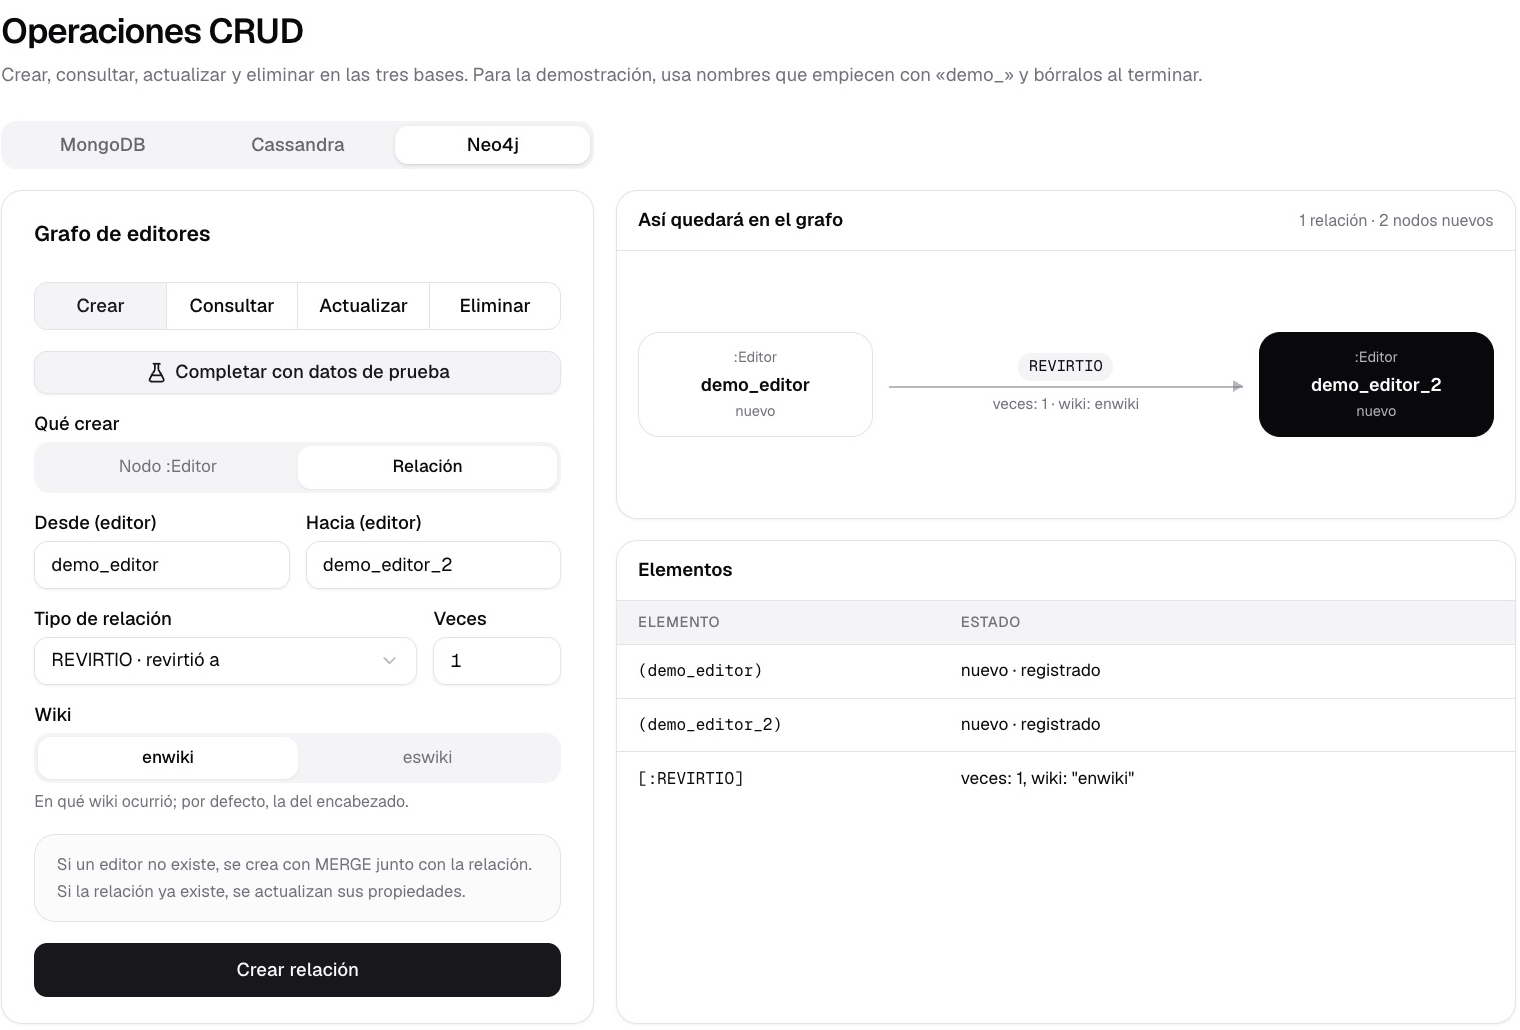
\includegraphics[width=0.96\textwidth,height=0.60\textheight,keepaspectratio]{dashboard-crud-neo4j.png}
\caption{Neo4j: creación de relaciones y vista previa del grafo.}\label{fig:ui-neo4j}
\fuente{dashboard del proyecto desplegado en Google Cloud Platform}
\end{figure}

\begin{tabla}
\begin{tabularx}{\textwidth}{P{2.2cm}YYY}
\toprule
Operación & MongoDB & Cassandra & Neo4j \\
\midrule
Crear & Insertar documento. & Insertar o reemplazar fila. & Crear nodo o relación. \\
Consultar & Leer documento o búsqueda filtrada. & Leer partición o clave completa. & Leer nodo, vecinos y propiedades. \\
Actualizar & Cambiar campos y recalcular derivados. & Cambiar valor o detalle. & Cambiar propiedades. \\
Eliminar & Borrar documento por identificador. & Borrar fila o partición. & Borrar una relación o nodo con sus relaciones. \\
\bottomrule
\end{tabularx}
\caption{Correspondencia funcional de las operaciones CRUD.}
\end{tabla}

La demostración por consola se ejecuta con \codigo{python -m wikipipe.crud todo}. Crea entidades de prueba, consulta el resultado, las modifica y las retira. No se ejecutó sobre una instalación productiva durante la elaboración de este informe.

\section{Vistas analíticas y operativas}
\subsection{Resumen y KPIs}
Presenta dos períodos: última hora consolidada y acumulado hasta un cierre identificado. Las cuatro tarjetas principales se complementan con detalles, protagonistas, evolución por hora y ejecuciones. Los protagonistas de la hora usan exclusivamente esa ventana. En el acumulado, los porcentajes se obtienen a partir de totales, evitando promediar porcentajes horarios.

Hay una diferencia entre el KPI histórico \codigo{total_eventos_acumulados}, que cuenta documentos de MongoDB anteriores al cierre, y las tarjetas acumuladas de la versión actual, que suman únicamente horas completadas del modelo 2. Sus cifras pueden diferir si existen eventos almacenados en ventanas todavía no consolidadas.

\subsection{En vivo}
Muestra eventos y participación de los últimos cinco minutos frente a los cinco anteriores. Ambos intervalos comparten un único instante de corte y no se superponen. Las tarjetas de editores cuentan participantes distintos en cada intervalo, no usuarios conectados a Wikipedia. La serie de treinta minutos aporta contexto y los filtros permiten revisar tipos, cuentas y borrados grandes.

La vista combina documentos y conteos provisionales. No debe compararse como si representara una hora completa ni interpretarse como una medición de latencia garantizada.

\subsection{Actividad en el tiempo}
Presenta el día local con horas consolidadas, evolución por minuto y páginas activas. Los eventos pendientes se informan aparte. El promedio por minuto divide entre el número de horas consolidadas multiplicado por 60, incluidos los minutos sin eventos. La comparación diaria utiliza las mismas horas del día anterior cuando la cobertura permite hacerlo.

\subsection{Explorador de eventos}
Consulta MongoDB y muestra composición por tipo sobre todo el dataset de las wikis elegidas. El total y los tipos salen de una misma agregación. Los filtros de búsqueda restringen la tabla de resultados, sin cambiar ese resumen general. La ficha permite revisar JSON y campos derivados.

\subsection{Red de editores}
Combina tarjetas de las últimas 24 horas hasta el cierre disponible con rankings de todo el historial conservado y la red alrededor de una cuenta. Los textos identifican esos alcances distintos. Se visualizan reversiones, mensajes, agradecimientos, bloqueos y coedición. La vista actual no presenta el ranking de páginas disputadas, aunque una consulta relacionada permanece disponible en la API.

\subsection{Operaciones CRUD y Arquitectura}
CRUD reúne formularios, previsualización y resultados de las tres bases. Arquitectura muestra componentes, conexiones y explicaciones de la fuente, almacenamiento, API y proceso horario. Sus pestañas permiten alternar el diagrama del despliegue y el funcionamiento lógico. Estas vistas facilitan la demostración técnica y la inspección del sistema.

\begin{tabla}
\begin{tabularx}{\textwidth}{P{3.5cm}P{3.7cm}Y}
\toprule
Vista & Fuente predominante & Período principal \\
\midrule
Resumen y KPIs & Cassandra, control en MongoDB y protagonistas de grafo/documentos. & Hora consolidada o acumulado al corte. \\
En vivo & MongoDB y minutos de Cassandra. & Cinco minutos; serie de treinta minutos. \\
Actividad & Cassandra y ventanas completadas. & Día local con horas consolidadas. \\
Explorador & MongoDB. & Dataset almacenado y búsqueda. \\
Red de editores & Neo4j y resúmenes de Cassandra. & Tarjetas de 24 h; rankings históricos. \\
CRUD & Las tres bases. & Registro o entidad seleccionada. \\
Arquitectura & Código y metadatos de las bases. & Estado y diseño del sistema. \\
\bottomrule
\end{tabularx}
\caption{Fuentes y alcance temporal de las siete vistas.}
\end{tabla}

\Needspace{18cm}
\section{Capturas y lectura de la interfaz}
Las figuras de este capítulo se obtuvieron del dashboard del proyecto desplegado en Google Cloud Platform, disponible en la dirección de la aplicación~\cite{dashboard}. Muestran los formularios CRUD y el recorrido de los datos entre los componentes del sistema.

\begin{figure}[H]
\centering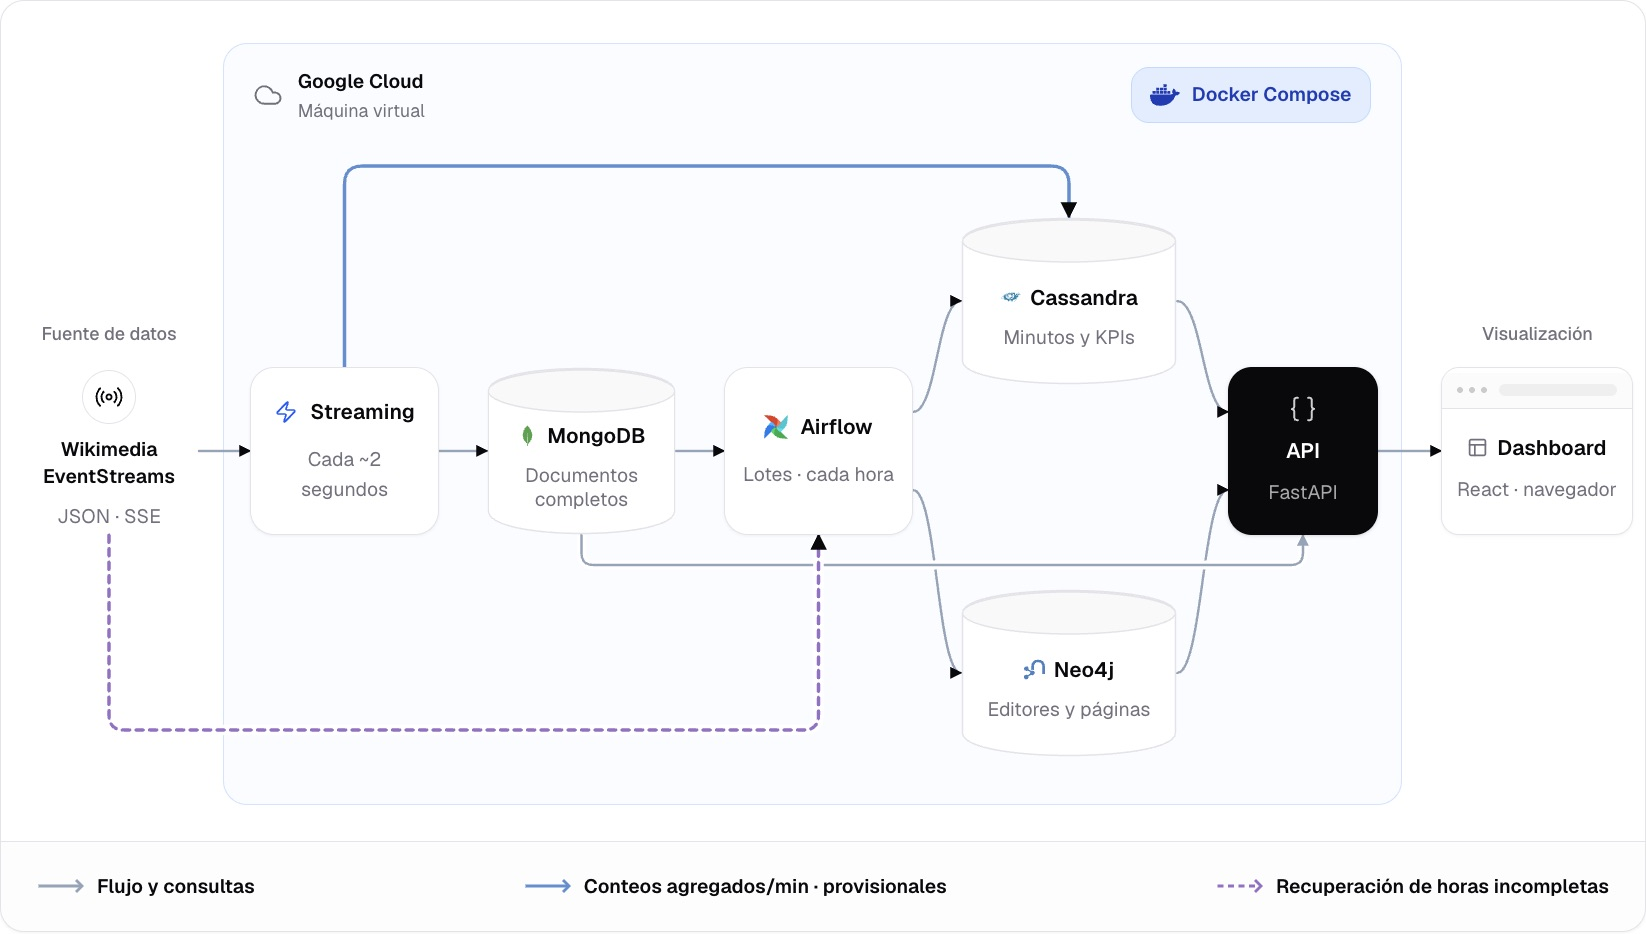
\includegraphics[width=\textwidth]{dashboard-arquitectura.png}
\caption{Arquitectura: recorrido de los datos y componentes del sistema.}\label{fig:ui-arq}
\fuente{dashboard del proyecto desplegado en Google Cloud Platform}
\end{figure}

La vista distingue tres recorridos: ingesta continua, consolidación horaria y consulta. Las flechas identifican los conteos provisionales y la recuperación de ventanas incompletas. Los componentes abren explicaciones de su función, mientras las pestañas permiten alternar la infraestructura y el proceso lógico.

\chapter{INDICADORES IMPLEMENTADOS}
\label{cap:kpis}
\section{Convenciones de cálculo}
Los doce KPIs se implementan en \ruta{src/wikipipe/kpis.py}. Se calculan para ambas wikis y para cada una por separado. Los resultados se almacenan como valor y detalle en \codigo{kpis} o \codigo{kpis_por_wiki}. El detalle identifica la entidad ganadora cuando el indicador representa una página o editor \cite{repo}.

Para una hora $h$, sean $E_h$ el total de eventos, $B_h$ los eventos de bots, $H_h$ los eventos humanos, $U_h$ los nombres humanos distintos, $M_h$ los eventos \codigo{edit}, $N_h$ los eventos \codigo{new}, $R_h$ las ediciones que contienen una reversión detectada y $V_h$ las entradas aceptadas únicas. $I_h$ representa las entradas del archivo de limpieza. Se utiliza $t_e$ para el instante \codigo{meta.dt} de un evento.

Una división sin denominador válido devuelve un valor ausente, no un cero. Las comparaciones entre porcentajes se muestran en puntos porcentuales. El frontend solo calcula diferencias horarias si los puntos son contiguos; así no confunde una hora faltante con una comparación inmediata.

\section{Volumen y evolución}
\subsection{Eventos de la hora}
\textbf{Definición:} número de eventos de los cuatro tipos procesados en la ventana. \textbf{Fórmula:}
\[
K_1(h)=E_h.
\]
\textbf{Fuente:} suma de \codigo{eventos} en \codigo{resumen_por_hora} de Cassandra. \textbf{Interpretación:} describe carga de actividad y de procesamiento. Una caída puede tener causas comunitarias, temporales o de cobertura; necesita contrastarse con el estado del pipeline.

\subsection{Cambio frente a la hora anterior}
\textbf{Definición:} variación porcentual del volumen respecto de la hora previa. \textbf{Fórmula:}
\[
K_2(h)=100\frac{E_h-E_{h-1}}{E_{h-1}}.
\]
\textbf{Fuente:} Cassandra. \textbf{Interpretación:} permite detectar cambios de ritmo. Si la hora anterior no existe o tiene cero eventos, el indicador queda ausente. Una variación positiva no representa por sí sola una mejora de calidad.

\subsection{Eventos acumulados}
\textbf{Definición:} documentos almacenados de las wikis elegidas anteriores al cierre de la hora. \textbf{Fórmula:}
\[
K_8(h)=\left|\{e\in\texttt{events}:t_e<h+1\text{ hora}\}\right|.
\]
\textbf{Fuente:} conteo filtrado de MongoDB. \textbf{Interpretación:} volumen histórico disponible hasta el corte. A diferencia del acumulado de las tarjetas actuales, este KPI no restringe el conteo a las ventanas publicadas del modelo 2. La distinción debe mantenerse al comparar cifras.

\section{Participación, automatización y creación}
\subsection{Proporción de eventos de bots}
\textbf{Definición:} participación de eventos automáticos entre todos los tipos. \textbf{Fórmula:}
\[
K_3(h)=100\frac{B_h}{E_h}.
\]
\textbf{Fuente:} Cassandra, usando la clasificación de la limpieza. \textbf{Interpretación:} cuantifica automatización del flujo observado. No es la proporción de cuentas bot ni únicamente de ediciones de artículos. Su exactitud depende de la clasificación de nombres y marcas.

\subsection{Actividad por editor humano}
\textbf{Definición:} promedio de eventos por nombre humano distinto durante la hora. \textbf{Fórmula:}
\[
K_4(h)=\frac{H_h}{|U_h|}.
\]
\textbf{Fuente:} agregación en MongoDB. \textbf{Interpretación:} intensidad de participación. El cálculo global obtiene los nombres distintos después de combinar las wikis; no suma cantidades de usuarios por wiki porque una misma cuenta podría aparecer en ambas. Incluye cuentas registradas, temporales e IP clasificadas como humanas y eventos de todos los tipos.

\subsection{Proporción de páginas nuevas}
\textbf{Definición:} creaciones entre ediciones y creaciones. \textbf{Fórmula:}
\[
K_5(h)=100\frac{N_h}{M_h+N_h}.
\]
\textbf{Fuente:} MongoDB. \textbf{Interpretación:} contrasta creación de páginas con mantenimiento. El denominador excluye categorizaciones y registros; una ``página'' puede pertenecer a espacios distintos al de artículos, pues no se impone \codigo{namespace=0} en este KPI.

\subsection{Variación neta de contenido}
\textbf{Definición:} bytes agregados menos bytes eliminados en \codigo{edit} y \codigo{new}. \textbf{Fórmula:}
\[
K_6(h)=\sum_{e\in W_h,\;type(e)\in\{edit,new\}}
\left(\operatorname{length.new}(e)-\operatorname{length.old}(e)\right).
\]
\textbf{Fuente:} MongoDB y \codigo{derived.delta_bytes}. Los tamaños ausentes se sustituyen por cero según la regla implementada. \textbf{Interpretación:} indica expansión o reducción neta; no mide calidad, importancia ni texto original. Un valor negativo puede responder a limpieza legítima, reversiones u otras modificaciones.

\section{Reversiones y relaciones}
\subsection{Ediciones que revierten}
\textbf{Definición:} porcentaje de eventos \codigo{edit} que revierten a otro editor según el comentario. \textbf{Fórmula:}
\[
K_7(h)=100\frac{R_h}{M_h}.
\]
\textbf{Fuente:} MongoDB. \textbf{Interpretación:} frecuencia observada de revisión por reversión. El denominador no incluye \codigo{new}. Depende de una heurística y no proporciona precisión o exhaustividad demostradas frente a todas las reversiones reales.

\subsection{Página más disputada}
\textbf{Definición:} página con mayor número de reversiones detectadas en la hora. Para cada página $p$ se cuenta $r_h(p)$:
\[
K_9(h)=\operatorname*{arg\,max}_{p}\ r_h(p).
\]
\textbf{Fuente:} primer puesto de \codigo{paginas_disputadas_por_hora} en Cassandra, comparado entre wikis cuando se combinan. El valor guarda la cantidad y el detalle la clave de página. \textbf{Interpretación:} prioriza inspección de páginas con actividad de reversión. No corresponde al antiguo criterio de cantidad de editores que aparece en mediciones iniciales.

\subsection{Editor humano más conectado}
\textbf{Definición:} cuenta humana con mayor cantidad de otros humanos que editaron páginas comunes dentro de la hora. Si $C_h(u)$ es ese conjunto:
\[
K_{10}(h)=\operatorname*{arg\,max}_{u\text{ humano}}|C_h(u)|.
\]
\textbf{Fuente:} Neo4j, recorrido \codigo{Editor-EDITO-Pagina-EDITO-Editor}, con hora y wiki cuando corresponde. Se cuentan vecinos distintos. \textbf{Interpretación:} centralidad de coactividad. El recorrido no demuestra acuerdo entre los participantes y no utiliza la relación acumulada \codigo{COEDITA} para producir el KPI horario.

\subsection{Editor más revertido}
\textbf{Definición:} cuenta que recibió más reversiones en la hora. \textbf{Fórmula:}
\[
K_{11}(h)=\operatorname*{arg\,max}_{u}\sum_{v}r_h(v,u).
\]
\textbf{Fuente:} Neo4j, suma de \codigo{veces} en relaciones entrantes \codigo{REVIRTIO}. El detalle incluye la cuenta y el número de editores que la revirtieron. \textbf{Interpretación:} señal para revisar la interacción en contexto, sin atribuir intención o vandalismo de forma automática.

\section{Calidad del procesamiento}
\subsection{Validación de eventos}
\textbf{Definición:} proporción de entradas que terminan como eventos válidos únicos. \textbf{Fórmula:}
\[
K_{12}(h)=100\frac{V_h}{I_h}.
\]
\textbf{Fuente:} estadísticas de \codigo{clean_file}. \textbf{Interpretación:} cumplimiento de reglas sobre el archivo procesado. Los duplicados reducen el numerador relativo; los rechazos tienen motivo explícito. El valor por wiki usa sus propias entradas y aceptados. Un archivo vacío produce valor ausente.

\section{Uso correcto de los períodos}
Los KPIs horarios no deben sumarse o promediarse sin considerar su significado. Los eventos, creaciones, reversiones y bytes pueden acumularse sobre ventanas disjuntas. Los porcentajes deben recalcularse con numeradores y denominadores totales. Los editores distintos requieren una nueva operación de distinción; sumar conteos horarios repite cuentas.

Para los protagonistas acumulados, la API consulta las ventanas completadas hasta el mismo corte y calcula los resultados desde MongoDB y Neo4j. No suma únicamente los ganadores horarios ni los rankings truncados: un candidato que nunca ganó una hora podría ser el primero en el acumulado.

Por ejemplo, si una hora tiene 1 evento de bot entre 2 eventos y otra tiene 10 entre 100, el promedio simple es 30\,\%, pero la proporción acumulada correcta es $11/102=10.78$\,\%. Esta diferencia explica por qué el dashboard conserva totales y períodos explícitos.

\chapter{RESULTADOS, DISCUSIÓN Y CONCLUSIONES}
\label{cap:resultados}
\section{Resultados documentados de procesamiento}
La evaluación combina los registros del equipo con las verificaciones locales realizadas para el informe. Las mediciones de la tabla~\ref{tab:evidencia} pertenecen a cortes diferentes y no se agregan como si procedieran de una misma ejecución.

\begin{tabla}
\begin{tabularx}{\textwidth}{P{3.2cm}P{4.0cm}Y}
\toprule
Evidencia y período & Resultado registrado & Alcance \\
\midrule
Captura exploratoria, 31 oct. & 4\,915 eventos en 134 s; 93 wikis. & Caracterización de la fuente global, previa al filtro final. \\
Dos horas, 31 oct. & 16\,442 y 15\,402 eventos; 31\,844 acumulados. & Primer procesamiento real de enwiki y eswiki. \\
CRUD en VM, registro del 31 oct. & Las 12 operaciones terminaron; se consultaron 79\,521 eventos. & Evidencia histórica de ejecución y superación del mínimo. \\
Comparación de fuentes, 12 nov. & 1\,598 identificadores iguales; 0 diferencias. & Ventana de cinco minutos, no todo el historial. \\
Reconstrucción, 17 nov. & 206\,762 eventos conservados desde las 01:00 UTC. & Corte reportado tras migrar al modelo 2. \\
\bottomrule
\end{tabularx}
\caption{Evidencias históricas con su período y alcance.}\label{tab:evidencia}
\fuente{\ruta{docs/trazabilidad.md} y \ruta{docs/justificacion-dataset.md}}
\end{tabla}

En las dos horas iniciales, el volumen pasó de 16\,442 a 15\,402 eventos, una disminución de aproximadamente 6.33\,\%. Las tasas de automatización registradas fueron 27.31\,\% y 27.22\,\%. Estos resultados ilustran los cálculos del sistema inicial; no acreditan los valores de una hora actual ni los rankings horarios del nuevo modelo.

La bitácora describe una repetición de la primera hora: MongoDB insertó cero documentos nuevos y el acumulado permaneció en 31\,844. Es una evidencia histórica de deduplicación. El modelo 2 amplía esa estrategia con reemplazo de contribuciones, correcciones y eliminación de filas obsoletas \cite{bitacora,correcciones}.

\section{Tiempos observados y límites de comparación}
En una ventana inicial de aproximadamente 16\,000 eventos se registraron 2.4 s para MongoDB, 4.3 s para Cassandra, 28 s para Neo4j y 1.7 s para KPIs. Estas cifras corresponden a etapas y versión iniciales; las tareas de Cassandra y Neo4j pueden correr en paralelo, de modo que su suma no es la duración del DAG \cite{bitacora}.

El 12 de noviembre se comparó la misma ventana de cinco minutos: MongoDB devolvió 1\,598 eventos en 0.2 s y EventStreams en 48.9 s, con igualdad de identificadores. Para esa muestra, el cociente de tiempos fue $48.9/0.2=244.5$. No se interpreta como aceleración universal: incluye acceso remoto, reproducción del stream y una única ventana. Otra ejecución documentada leyó 20\,770 eventos desde MongoDB en 3.2 s; la hora anterior, recuperada externamente, tuvo un volumen y duración diferentes \cite{bitacora}.

La frecuencia de vaciado de dos segundos no garantiza que cada evento aparezca en pantalla en ese plazo. La latencia total incluye recepción, persistencia, conteos, consultas y refresco. No se realizó para este informe un experimento de percentiles de latencia ni una prueba de carga sostenida.

\section{Migración temporal y recorte del historial}
La integración del modelo 2 detectó relaciones antiguas sin atribución horaria. El código rechazó la carga para impedir mezclar ambos formatos. La bitácora registra que se conservó un snapshot y se optó por reconstruir un período reducido en lugar de reprocesar las aproximadamente 400 horas del historial anterior \cite{bitacora}.

Se eliminaron los eventos anteriores al 17 de noviembre y se reconstruyeron las tablas derivadas y el grafo. La hora 00:00 UTC, con 57\,669 eventos y fuerte concentración de actividad en un bot, quedó excluida después de bloquear una carga de Neo4j durante más de veinte minutos. Las demás horas reconstruidas se reportaron alrededor de veinte segundos cada una. El corte posterior registró 206\,762 eventos y catorce horas reconstruidas de 01:00 a 14:00 UTC; la hora de las 15:00 se recuperó posteriormente mediante el DAG.

Esta decisión mantiene un volumen superior al mínimo del curso, pero reduce la cobertura y elimina precisamente una hora de alta actividad automática. Por ello, el dataset conservado no representa un día completo ni una muestra aleatoria del día. El incidente es evidencia de un límite de escalabilidad de la transacción horaria del grafo y debe acompañar cualquier interpretación de volumen o automatización.

\section{Verificación ejecutada para el informe}
Se ejecutaron las pruebas existentes en un entorno Python 3.11 con las versiones fijadas de los drivers de la API. El resultado fue \textbf{19 pruebas correctas y un módulo omitido}. El módulo de integración se omite deliberadamente si \codigo{WIKIPIPE_INTEGRATION} no vale 1; contiene diez pruebas que necesitan los tres motores. Docker estaba detenido en el equipo, por lo que no se presentan como ejecutadas en esta revisión \cite{verificacion}.

\begin{tabla}
\begin{tabularx}{\textwidth}{P{4.3cm}P{2.8cm}Y}
\toprule
Verificación & Resultado & Qué comprueba \\
\midrule
Python: limpieza & 11 pruebas correctas. & Tipos de usuario, validación, derivados, comentarios y registros malformados. \\
Python: decisión de fuente & 4 pruebas correctas. & Cobertura completa, huecos, espera y tramo detenido. \\
Python: streaming & 4 pruebas correctas. & Filtro, contadores, rechazos y cobertura en vivo. \\
Integración con bases & Módulo omitido. & Requiere MongoDB, Cassandra y Neo4j activos; diez casos definidos. \\
Renderizado React & Correcto. & Períodos, unidades, acumulados, datos vacíos y textos. \\
Historial CRUD en frontend & Correcto. & Orden, datos actualizados, registros borrados y errores temporales. \\
Compilación del frontend & Correcta. & TypeScript y construcción de producción con Vite. \\
\bottomrule
\end{tabularx}
\caption{Resultado y alcance de las verificaciones locales.}
\end{tabla}

Las pruebas de integración disponibles abarcan reemplazo y aislamiento temporal, distinción de cuentas entre wikis, fallos y reinicios de streaming, marcas de escritura, operaciones CRUD, eliminación exacta de relaciones, rollback del grafo, paginación y alcances de vistas. Su existencia aporta cobertura prevista; la bitácora registra una ejecución previa en desarrollo, pero esta revisión no la sustituye por un resultado nuevo.

\section{Discusión de limitaciones}
\begin{itemize}
\item \textbf{Escala y disponibilidad.} Los servicios comparten una VM y Cassandra tiene replicación 1. Una falla del host afecta al conjunto. El modelo de consultas es compatible con crecimiento, pero la instalación actual no demuestra escalabilidad distribuida.
\item \textbf{Concentración del grafo.} La transacción de reemplazo y la reconstrucción acumulada pueden encarecer una ventana con cuentas de mucha actividad. El mutex global también serializa las cargas del grafo.
\item \textbf{Cobertura y retención.} Los márgenes temporales y la recuperación externa son políticas operativas con historial limitado. El recorte documentado deja una ausencia conocida que debe hacerse visible al analizar el día.
\item \textbf{Inferencias.} Bots, reversiones y categorías dependen parcialmente de nombres o comentarios. No se dispone de una medición independiente de precisión y exhaustividad.
\item \textbf{Consistencia.} Las bases se actualizan en etapas. La publicación por ejecución y la verificación de versión reducen lecturas mixtas, pero no aportan atomicidad distribuida. Las modificaciones CRUD requieren reconstrucción de derivados.
\item \textbf{Seguridad y mantenimiento.} La contraseña compartida y el despliegue automático cubren una demostración; quedan pendientes roles, TLS, migraciones previas y una estrategia de respaldo y restauración integral.
\end{itemize}

\section{Conclusiones}
El proyecto implementa el recorrido completo desde eventos semiestructurados de Wikipedia hasta consultas documentales, series temporales y relaciones entre entidades. La distribución de responsabilidades aprovecha MongoDB para conservar contexto y reconstruir, Cassandra para leer materializaciones temporales y Neo4j para expresar conexiones. Los tres motores tienen una función verificable en el código y el dashboard.

El DAG satisface las seis etapas solicitadas y añade recuperación desde la fuente externa cuando falta cobertura local. La versión temporal incorpora claves estables, ventanas semiabiertas, bloqueo renovable, marcas crecientes, manifiestos y reemplazo transaccional del grafo. Estos mecanismos explican cómo se busca evitar duplicados y reconstruir resultados, sin atribuir al sistema una consistencia distribuida que no implementa.

Los doce KPIs y las siete vistas permiten observar volumen, automatización, creación, revisión y participación. Su utilidad depende de respetar denominadores, cortes y alcances: un conteo provisional de cinco minutos no es una hora consolidada, y una relación de coedición no demuestra colaboración intencional.

La cifra documentada de 206\,762 eventos después de la reconstrucción supera el mínimo académico. No obstante, la exclusión de la hora de mayor concentración revela una restricción real del grafo y limita la representatividad del período. La solución cumple el alcance funcional implementado, mientras que su operación prolongada exige mejorar escalabilidad, cobertura, seguridad y procedimientos de migración.

\section{Trabajo futuro}
Se propone priorizar cargas de grafo con un área de preparación y publicación por versión, para acotar transacciones sin perder coherencia por ventana; evaluar estas cargas con distribuciones reales y cuentas muy activas; y reconstruir la hora excluida cuando exista una ruta de procesamiento validada.

También conviene segmentar las particiones históricas de Cassandra, incorporar política de retención y restauración probada de las tres bases, medir latencia y frescura por percentiles, y ejecutar las regresiones de integración antes de desplegar cambios de modelo. Para el análisis, un corpus de reversiones etiquetadas permitiría evaluar la heurística. Las relaciones de creación, categorías, traslados y archivos pueden alimentar indicadores temáticos adicionales.

\cleardoublepage
\phantomsection\addcontentsline{toc}{chapter}{Referencias bibliográficas}
\renewcommand{\bibname}{REFERENCIAS BIBLIOGRÁFICAS}
\bibliographystyle{IEEEtran}
\begingroup
\setstretch{1.05}\small\raggedright
\bibliography{referencias}
\endgroup
\begingroup
\small\setstretch{1.08}
\appendix
\renewcommand{\thechapter}{\Alph{chapter}}
\renewcommand{\thesection}{\Alph{chapter}.\arabic{section}}
\renewcommand{\thetable}{\Alph{chapter}.\arabic{table}}
\renewcommand{\thefigure}{\Alph{chapter}.\arabic{figure}}
\chapter{REPRODUCIBILIDAD Y TRAZABILIDAD}
\section{Mapa del repositorio}
\begin{tabla}
\begin{tabularx}{\textwidth}{P{4.3cm}Y}
\toprule
Ubicación & Responsabilidad revisada \\
\midrule
\ruta{src/wikipipe/extract.py}, \ruta{fuente.py} & Consumo SSE, recuperación y decisión de fuente horaria. \\
\ruta{src/wikipipe/clean.py}, \ruta{config.py} & Reglas, derivados y variables del pipeline. \\
\ruta{src/wikipipe/streaming.py}, \ruta{windows.py} & Ingesta, cobertura y coordinación de escrituras. \\
\ruta{src/wikipipe/mongo.py}, \ruta{cassandra_store.py}, \ruta{neo4j_store.py} & Persistencia, agregación y construcción temporal de relaciones. \\
\ruta{src/wikipipe/kpis.py}, \ruta{rebuild.py}, \ruta{crud.py} & Indicadores, reconstrucción y operaciones sobre las bases. \\
\ruta{db/}, \ruta{airflow/dags/} & Esquemas, restricciones, índices y DAG. \\
\ruta{api/}, \ruta{web/src/} & API y aplicación analítica. \\
\ruta{docker-compose.yml}, \ruta{infra/}, \ruta{deploy.sh}, \ruta{local.sh} & Ejecución local, infraestructura y despliegue. \\
\ruta{tests/}, \ruta{docs/} & Pruebas, guías, requisitos y evidencia histórica. \\
\bottomrule
\end{tabularx}
\caption{Guía de navegación del código fuente.}
\end{tabla}

\section{Ejecución local y esquemas}
Los siguientes comandos describen el procedimiento reproducible del repositorio. No indican que el entorno completo se haya levantado durante esta revisión.
\par\noindent\begin{minipage}{\linewidth}
\begin{lstlisting}
./local.sh
# Alternativa manual:
cp .env.example .env
# Configurar las variables y contraseñas antes del arranque.
docker compose up -d --build

docker compose exec airflow \
  python /opt/airflow/db/create_schemas.py
\end{lstlisting}
\end{minipage}\par

El dashboard se sirve en \codigo{http://localhost:8501}; Airflow en el puerto 8080 salvo configuración distinta; Neo4j Browser en 7474. La API de desarrollo se publica en \codigo{127.0.0.1:8010}. Las credenciales se toman de variables y no se incluyen en este documento.

\section{Procesamiento de una ventana y CRUD}
El ejemplo procesa una hora mediante el comando de prueba del DAG. Se debe verificar el intervalo asignado por Airflow en la ejecución; la guía local del repositorio utiliza la hora de cierre como referencia para estas demostraciones.
\par\noindent\begin{minipage}{\linewidth}
\begin{lstlisting}
docker compose exec airflow airflow dags test \
  wikipedia_recent_changes 2026-11-17T11:00:00+00:00

docker compose exec airflow python -m wikipipe.crud todo
\end{lstlisting}
\end{minipage}\par

Para una reconstrucción del modelo se deben seguir los pasos de \ruta{docs/correcciones-dev-ian.md}: copia recuperable, pausa del DAG, espera de tareas y detención de streaming. \codigo{--reset-graph} respalda el grafo en JSONL gzip y después lo vacía, incluidas entidades manuales. Este informe no ejecuta esa operación.

\section{Comandos de verificación}
\par\noindent\begin{minipage}{\linewidth}
\begin{lstlisting}
PYTHONPATH=src:api python -m pytest tests -q
node tests/test_dashboard.mjs
node tests/test_crud_history.mjs
npm run build --prefix web
\end{lstlisting}
\end{minipage}\par
La revisión usó Python 3.11.17 y un entorno temporal con las dependencias del repositorio y de la API, además de \codigo{pytest} y \codigo{httpx}. Las salidas y versiones se conservan en \ruta{informe/evidencias/verificacion.txt}.

Para habilitar las diez regresiones que requieren bases, la documentación proporciona este procedimiento en un proyecto Compose de desarrollo:
\par\noindent\begin{minipage}{\linewidth}
\begin{lstlisting}
docker compose -p wikipipe-dev-ian up -d --build
docker compose -p wikipipe-dev-ian cp tests/. api:/tmp/tests/
docker compose -p wikipipe-dev-ian exec -T api pip install pytest httpx
docker compose -p wikipipe-dev-ian exec -T \
  -e WIKIPIPE_INTEGRATION=1 api \
  python -m pytest /tmp/tests/test_pipeline_integration.py -q
\end{lstlisting}
\end{minipage}\par

Los tests de integración usan nombres temporales para MongoDB y Cassandra y prefijos para entidades de Neo4j. Deben ejecutarse en un entorno de desarrollo aislado. La muestra de \ruta{tests/seed_local.py} contiene 55\,000 registros sintéticos: sirve para probar procesamiento y no acredita el volumen real de Wikimedia.

\section{Correspondencia con el enunciado}
\begin{table}[H]\centering\small\setstretch{1.05}\renewcommand{\arraystretch}{1.2}
\begin{tabularx}{\textwidth}{P{3.8cm}P{2.3cm}Y}
\toprule
Requisito & Desarrollo en el informe & Evidencia principal \\
\midrule
Fuente semiestructurada y actualizable & Cap. II & JSON, SSE y consumidor continuo. \\
Mínimo de 50\,000 registros & Cap. II y VII & 206\,762 eventos documentados tras la reconstrucción. \\
Justificación multimodelo & Cap. III & Esquemas y patrones de consulta de las tres bases. \\
DAG programado de seis etapas & Cap. IV & Dependencias y configuración horaria. \\
CRUD en cada base & Cap. V & Funciones, API, interfaz y demo de consola. \\
Dashboard y capturas & Cap. V & Siete vistas; capturas del dashboard desplegado en GCP. \\
Cinco o más KPIs con fórmula e interpretación & Cap. VI & Doce indicadores implementados. \\
Conclusiones & Cap. VII & Resultados, límites y mejoras. \\
Código, scripts y DAG & Anexo A & Archivos y comandos del repositorio. \\
Video y evaluación de pares & Entregables complementarios & Su ejecución no se acredita mediante este informe. \\
\bottomrule
\end{tabularx}
\caption{Trazabilidad de los requisitos académicos.}
\end{table}

\section{Identificación y plantilla}
Código revisado: \texttt{\RevisionCodigo}. Las cifras históricas proceden de la bitácora; las descripciones técnicas siguen el código vigente. Se conservaron la clase \codigo{tesisutec.cls}, el estilo \codigo{IEEEtran.bst} y el logo de la plantilla. La portada se adaptó al curso y sus datos se editan en \ruta{datos.tex}.

\section{Alcance y método de revisión del informe}
Se revisaron el código Python del pipeline y la API, los esquemas JSON/CQL/Cypher, el DAG, el frontend TypeScript, los archivos de contenedores, Terraform, las pruebas y la documentación del repositorio. La referencia de esta revisión es el commit \texttt{\RevisionCodigo}, del 17 de noviembre de 2026 \cite{repo}.

La evidencia se distingue en tres grupos: comportamiento comprobable en el código, mediciones históricas registradas en la bitácora y verificaciones ejecutadas para este informe. No se interpreta una configuración de escritura cada dos segundos como una medición completa de latencia. Tampoco se presenta una prueba sintética como acreditación del dataset real.

El sistema opera en una VM, sin clúster ni alta disponibilidad. Sus resultados dependen de la retención, el tamaño de las transacciones y las reglas heurísticas.

\endgroup
\end{document}
